\chapter{Model Architecture}\label{mdlarc}
In this chapter, the architectures of several models are presented. Section \ref{modpoly} gives a comprehensive explanation to the structure of PolygonRNN, while section \ref{modfpn} gives basic concepts in both single and multiple bounding box(es) regression and looks into FPN.

Considering our problem, we combine PolygonRNN and FPN together and come up with a new model, which is called \modelnameshort\ (\modelnamelong, see section \ref{modmer}). In theory, the proposed model can find out the bounding boxes for buildings within an aerial image and give geometrical shape for each building.
 
\section{PolygonRNN}\label{modpoly}

PolygonRNN is the core model for exploiting geometrical shapes in this thesis project. Figure \ref{fig:simppoly} shows its simplified architecture, which consists of two parts. The CNN part (see subsection \ref{modcnn}) can capture image features through multilayer convolutions and maximum pooling. Those captured features are then fed into the RNN part (see subsection \ref{modrnn}), which sequentially predicts spatial location of the new vertex with the highest probability at each time step.

\begin{figure}[!h]
	\centering
	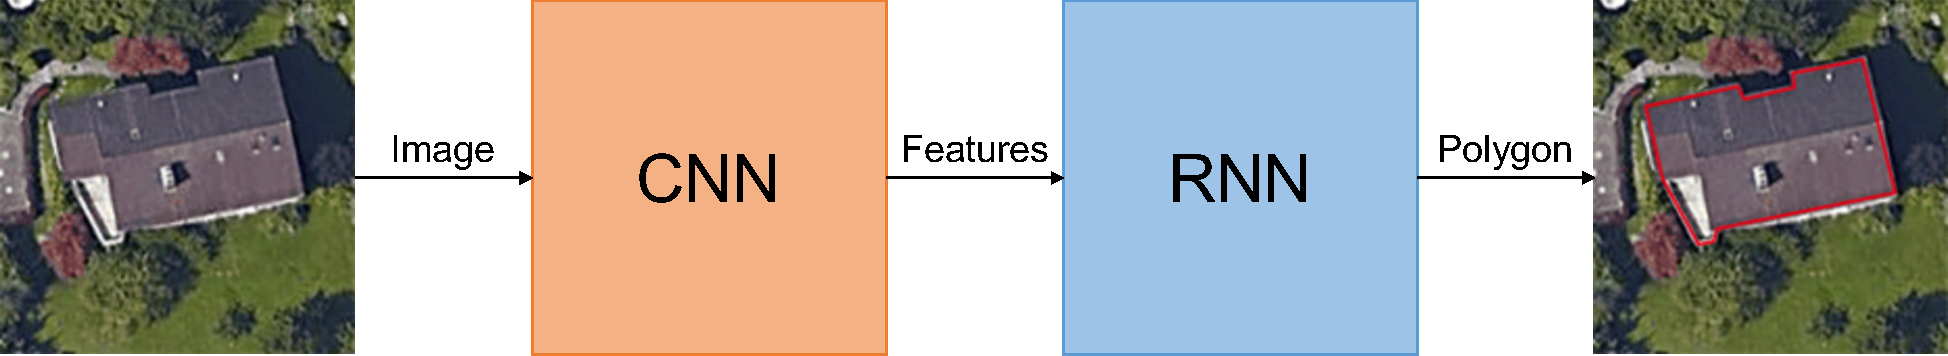
\includegraphics[width=\fig\textwidth]{3-00.pdf}
    \caption[The simplified model architecture of PolygonRNN]{The simplified model architecture of PolygonRNN.}
    \label{fig:simppoly}
\end{figure}

\subsection{CNN Part}\label{modcnn}
The CNN part of PolygonRNN uses VGG-16 \cite{vgg16}. Actually, VGG-16 is a form of VGGNet \cite{vgg16}, which is very structured and focusing on deepening the  neural network without a large number of parameters. It generally believes that deeper networks have stronger expressive capabilities than shallow networks, and can accomplish more complex tasks. It also proven in practice that VGGNet has made great progress in performance compared to its previous network architecture (e.g. AlexNet \cite{alexnet}).

The ``16" in VGG-16 means that it is a VGGNet with 16 layers containing parameters (13 convolutional layers and 3 fully connected layers). It has around 138 million parameters in total. Figure \ref{fig:vgg16} shows its detailed network structure. From the figure we can see that VGG-16 continuously does convolution with 3$\times$3 small kernels and makes 2$\times$2 maximum pooling. As the network deepens, the width and height of the image are reduced by half after each maximum pooling, and the number of channels is also doubly increasing after some convolutional layers.

\begin{figure}[!h]
	\centering
	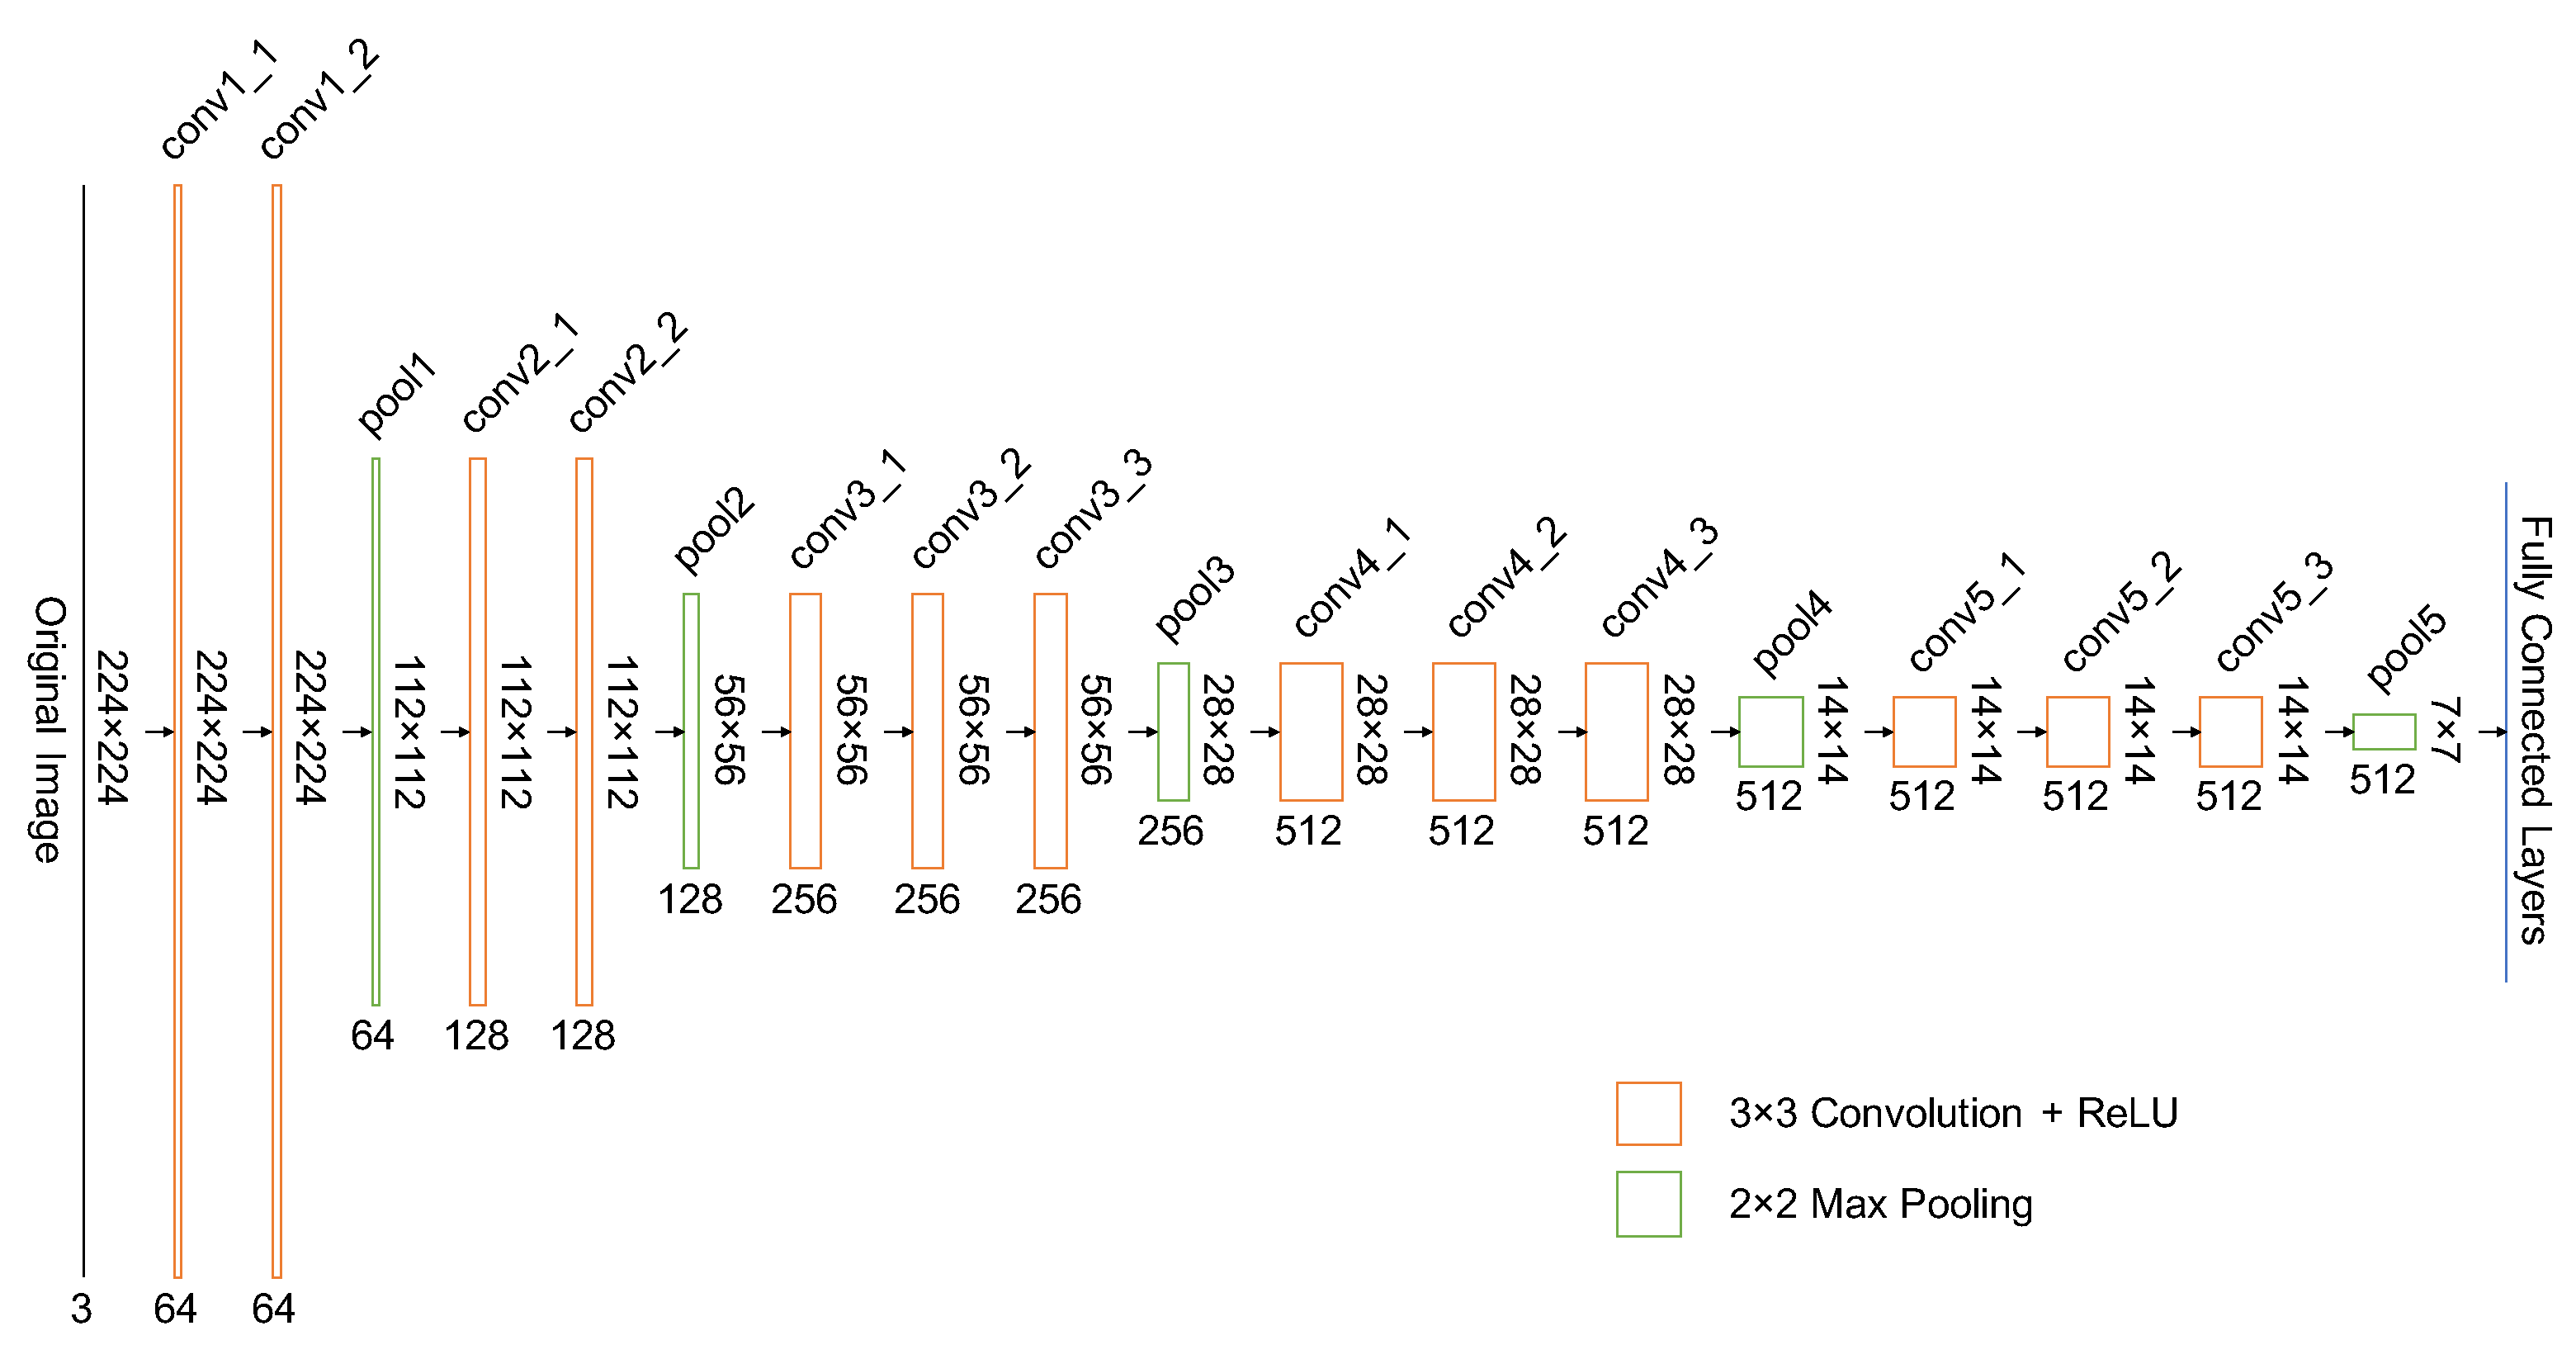
\includegraphics[width=\fig\textwidth]{3-01.pdf}
    \caption[VGG-16 architecture]{VGG-16 architecture. Only convolutional layers and maximum pooling layers are presented.}
    \label{fig:vgg16}
\end{figure}

VGG-16 was mostly used for image classification before. Hence, after the convolutional layers and maximum pooling layers, there are fully connected layers and softmax layer for the class labels. However, these two kinds of layers are not required for VGG-16 used in PolygonRNN, because the CNN here is working as a feature extractor and mask predictor. Layer \lstinline{pool5} is omitted as well because of the too low resolution.

\paragraph{Feature Extraction} The modified VGG-16 provides RNN with useful features, which are taken from different convolutional and maximum pooling layers. Thus, similar to FCN mentioned in subsection \ref{dlsemseg}, the network here also uses skip connection. Specifically, the features are extracted from layers \lstinline{pool2}, \lstinline{pool3}, \lstinline{conv4_3} and \lstinline{conv5_3}. Note that since the resolution of final features is fixed, when taking features from layer \lstinline{pool2} and \lstinline{conv5_3}, it requires another maximum pooling and upsampling respectively. All of these processes can be seen in figure \ref{fig:mdfvgg16}.

\begin{figure}[!h]
	\centering
	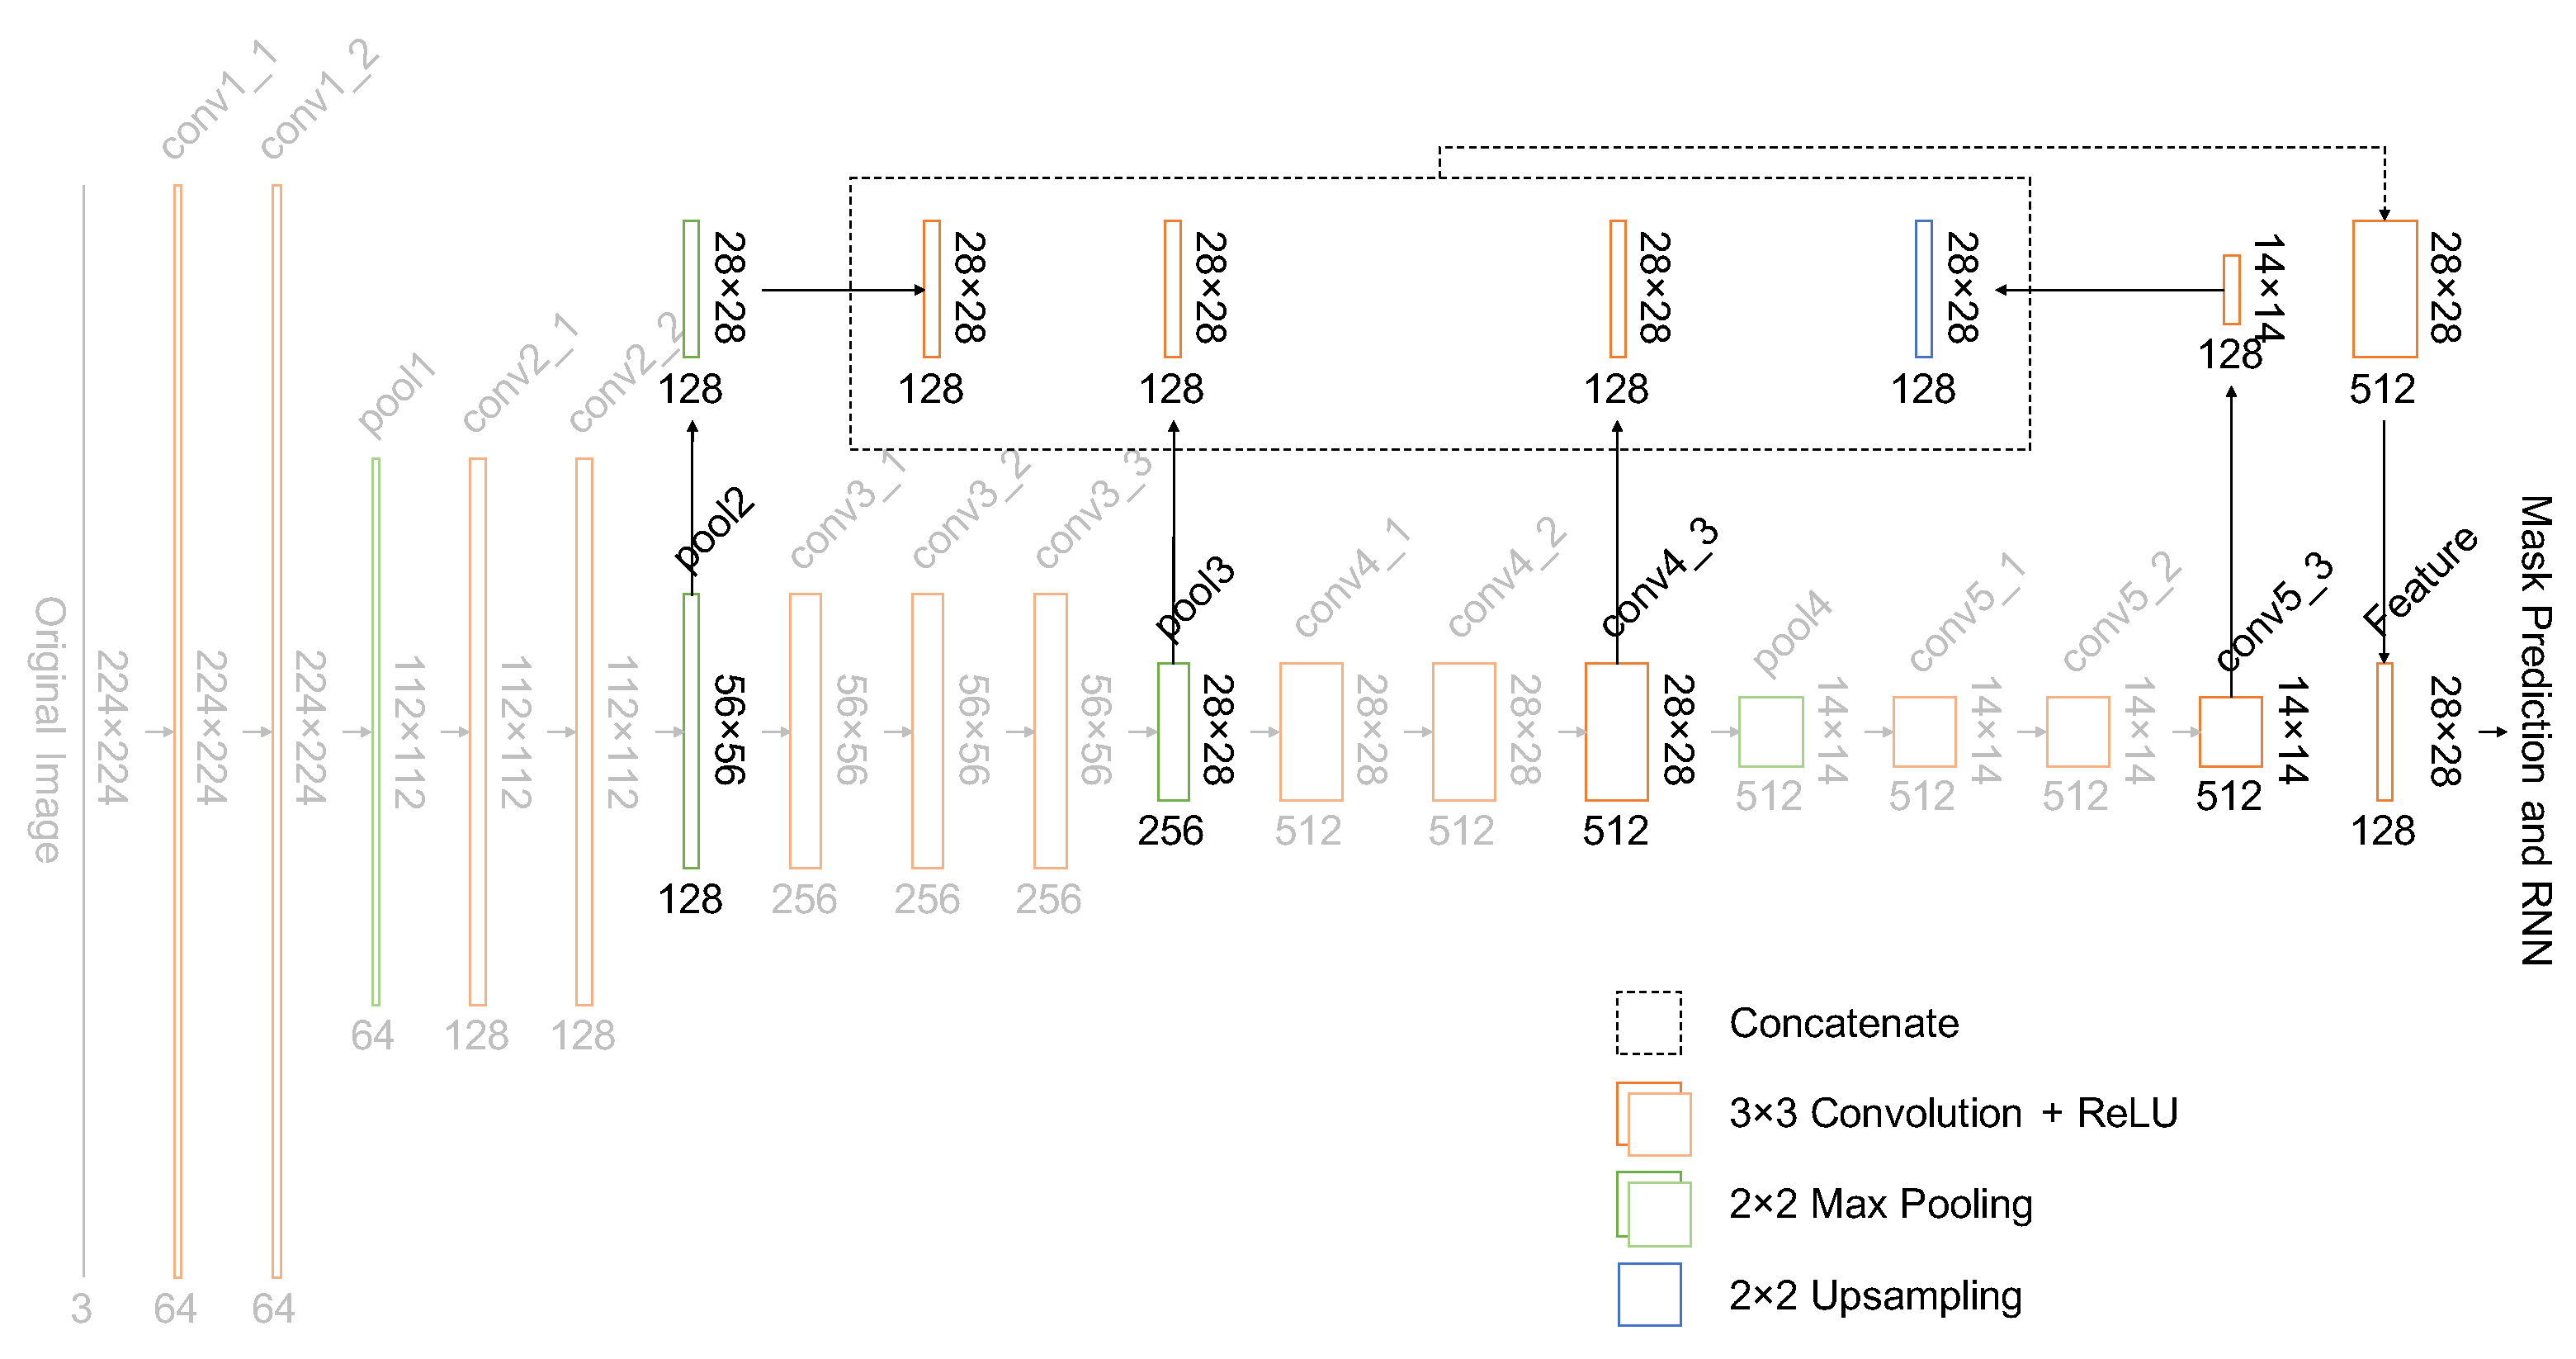
\includegraphics[width=\fig\textwidth]{3-02.pdf}
    \caption{Modified VGG-16 architecture in PolygonRNN.}
    \label{fig:mdfvgg16}
\end{figure}

\paragraph{Mask Prediction}
Another function of the CNN part is to predict masks of boundary and vertices in a low resolution (one eighth of the original). Figure \ref{fig:vgg16mask} shows the mask prediction phase. Different from the ReLU (Rectified Linear Units) \cite{relu} non-linearity used in the former convolutional layers, the activation function used here is the general sigmoid function.

\begin{figure}[!h]
	\centering
	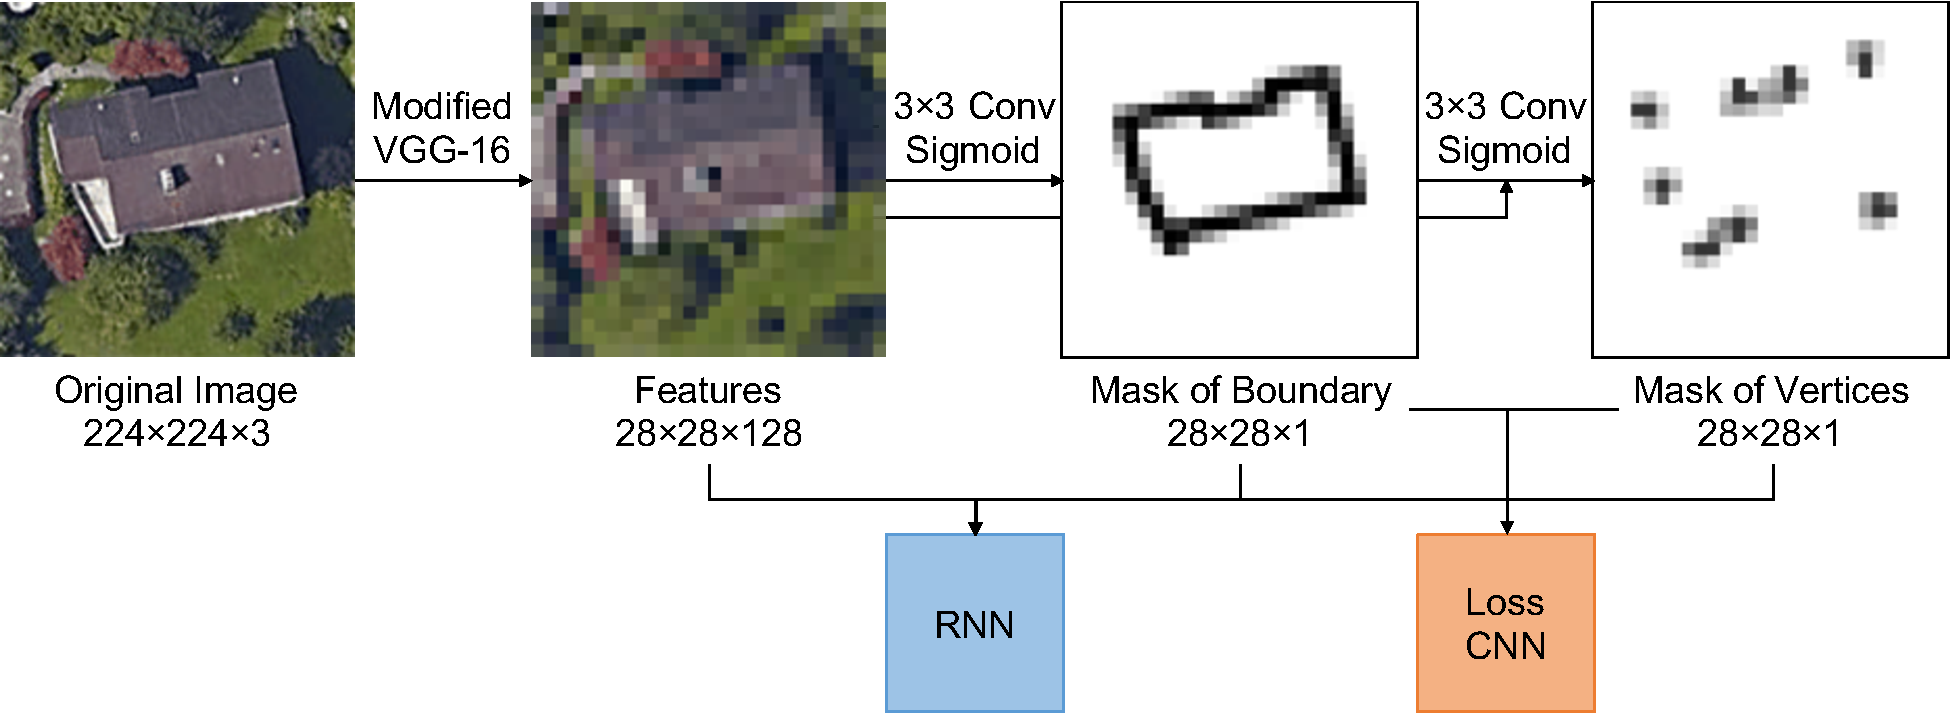
\includegraphics[width=\fig\textwidth]{3-03.pdf}
    \caption[Mask prediction of VGG-16]{Mask prediction of VGG-16. Note that the mask of vertices is obtained by the convolution on the concatenation of the features and the mask of boundary.}
    \label{fig:vgg16mask}
\end{figure}

Each entry of the boundary or the vertices mask indicates the probability that the pixel is located in the boundary or is a vertex, respectively. The features and two masks are then sent into RNN together. In addition, the two masks are used to calculate the loss of CNN part. For the loss function used here, please refer to subsection \ref{losspoly}.

\subsection{RNN Part}\label{modrnn}
The basic model used for predicting polygon vertices is RNN. We have already mentioned in subsection \ref{polygonrnn} that RNN is very powerful when data is related to time series, and in our case, we regards the polygon as a series of vertices.

As we know, given two adjacent vertices on a polygon in an specific order (either clockwise or anticlockwise), the third vertex after the two points can be uniquely determined. What RNN here can do is to predict the probability distribution of the next vertex's position when given the history information about the two vertices before. The calculation process also requires the image features and the position of the starting vertex, which is formulated as follows.
\begin{equation}\label{eq:vnext}
	P(v_t \mid v_{t-1}, v_{t-2}) = F(v_{t-1}, v_{t-2}, v_0, f), \forall t \in \{2,3,\ldots,T\},
\end{equation}
where $f$ denotes the extracted features by CNN (including both masks of boundary and vertices as well), $F(\cdot)$ denotes a function (actually the simulation of RNN) for computing the conditional probability, $T$ denotes the number of vertices of the polygon, $v_t$ denotes the vertex position at $t$-th prediction. Specifically, the vertex prediction problem can be formulated as a classification problem. The position of $v_t$ can be then quantized to the resolution of output grid, and we can thus use one-hot encoding for $v_t$'s representation.

\paragraph{End Signal} Note that the positions for $v_t$ are not only limited to the general output grid, the end signal for the closure detection of the polygon is also embedded in $v_t$'s assignments, just like the ``end of sequence" token \lstinline{<eos>} or \lstinline{</s>} in RNN language model. Thus, the number possible assignments of $v_t$ equals to the resolution of the output grid plus one ($28\times28+1=785$ in our case). In order to correctly predict the end signal, the starting vertex $v_0$ is required for the conditional probability (equation \ref{eq:vnext}) calculation, as it tells the model when to finish the prediction phase. If the current prediction is the same as, or very close to the starting vertex $v_0$, $v_t$ will be forced to raise the end signal, indicating that the entire polygon is close, and the prediction phase is therefore complete. So generally, the end signal works when $t=T$.

\paragraph{Starting Vertex} In equation \ref{eq:vnext}, two special cases $P(v_0)$ and $P(v_1 \mid v_0)$ are not included yet. These two cases are different from the general case, and should be considered in addition. In particular, we can directly regard the mask of vertices (for example, the rightmost image in figure \ref{fig:vgg16mask}) predicted by the CNN as $v_0$'s unnormalized probability distribution $\tilde{P}(v_0)$, and choose the position with the highest probability for $v_0$'s assignment. As $v_0$ is known, there are typically two options for $v_1$, one is the next vertex on its left direction and another on right direction. To tackle the problem of vertices ordering, we can simply specify the order of polygon vertices to be fixed, so that $v_1$ can be uniquely determined. In our project, the order of polygon is set to be anticlockwise, and in practice, we simply use equation \ref{eq:vsecond} to get the conditional probability distribution of $v_1$ given $v_0$.
\begin{equation}\label{eq:vsecond}
	P(v_1 \mid v_0) = F(v_0, v_0, v_0, f).
\end{equation}

\paragraph{ConvLSTM} The RNN uses ConvLSTM (Convolutional LSTM) \cite{convlstm} cells as the polygon decoder to sequentially predict vertices. For simplicity, we can regard ConvLSTM as the function $F(\cdot)$ in equations \ref{eq:vnext} and \ref{eq:vsecond}. In fact, the structure of a ConvLSTM cell is almost the same as that of an ordinary LSTM (Long Short-Term Memory) \cite{lstm} cell, except that it employs convolution in a 2D image with multiple channels instead of multiplication of matrices and vectors. The introduction of ConvLSTM can significantly reduce the the number of parameters when compared with a fully connected RNN. The following equations define the computation process within a ConvLSTM cell, which is also visualized in figure \ref{fig:lstmcell}.

\begin{figure}[!h]
	\centering
	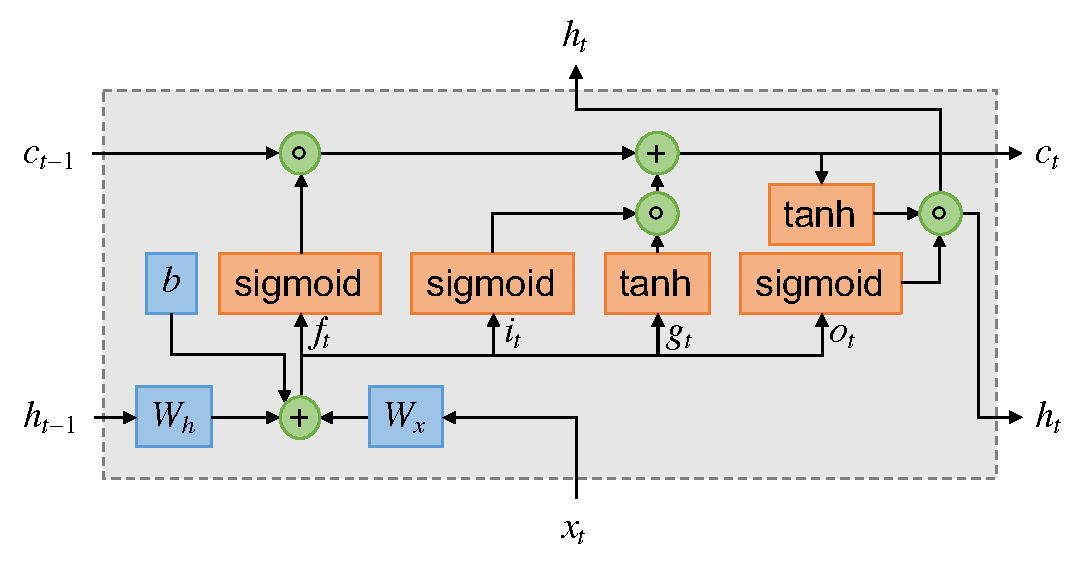
\includegraphics[width=\fig\textwidth]{3-04.pdf}
    \caption{Visulization for LSTM cell.}
    \label{fig:lstmcell}
\end{figure}

\begin{equation}
	\left[\begin{array}{c}
		f_t\\i_t\\g_t\\o_t
	\end{array}\right] = \left[\begin{array}{c}
		W_{hf}\\W_{hi}\\W_{hg}\\W_{ho}
	\end{array}\right] * h_{t-1} + \left[\begin{array}{c}
		W_{xf}\\W_{xi}\\W_{xg}\\W_{xo}
	\end{array}\right] * x_{t} + \left[\begin{array}{c}
		b_f\\b_i\\b_g\\b_o
	\end{array}\right] = W_h * h_{t-1} + W_x * x_t + b,
\end{equation}
\begin{equation}
	c_t = \sigma(f_t) \circ c_{t-1} + \sigma(i_t) \circ \tanh(g_t),
\end{equation}
\begin{equation}
	h_t = \sigma(o_t) \circ \tanh(c_t),
\end{equation}
where $x_t$, $h_t$, $c_t$ denote the input, the hidden state (or cell output), and the cell state of the cell at time step $t$ respectively, $i_t$, $o_t$, $f_t$ denote the states of input, output, and forget gate at time step $t$ respectively, $g_t$ denotes an intermediate variable, $\sigma(\cdot)$, $*$, $\circ$ denote the sigmoid function, convolution, and Hadamard (element-wise) product respectively, $W_x$ and $W_h$ denotes two convolution kernels for $x_t$ and $h_t$ respectively, $W_{xf}$, $W_{xi}$, $W_{xg}$, $W_{xo}$ denote the four components of $W_x$ in the dimension of channels and $W_{hf}$, $W_{hi}$, $W_{hg}$, $W_{ho}$ denote the four components of $W_h$ in the dimension of channels.

\begin{figure}[!h]
	\centering
	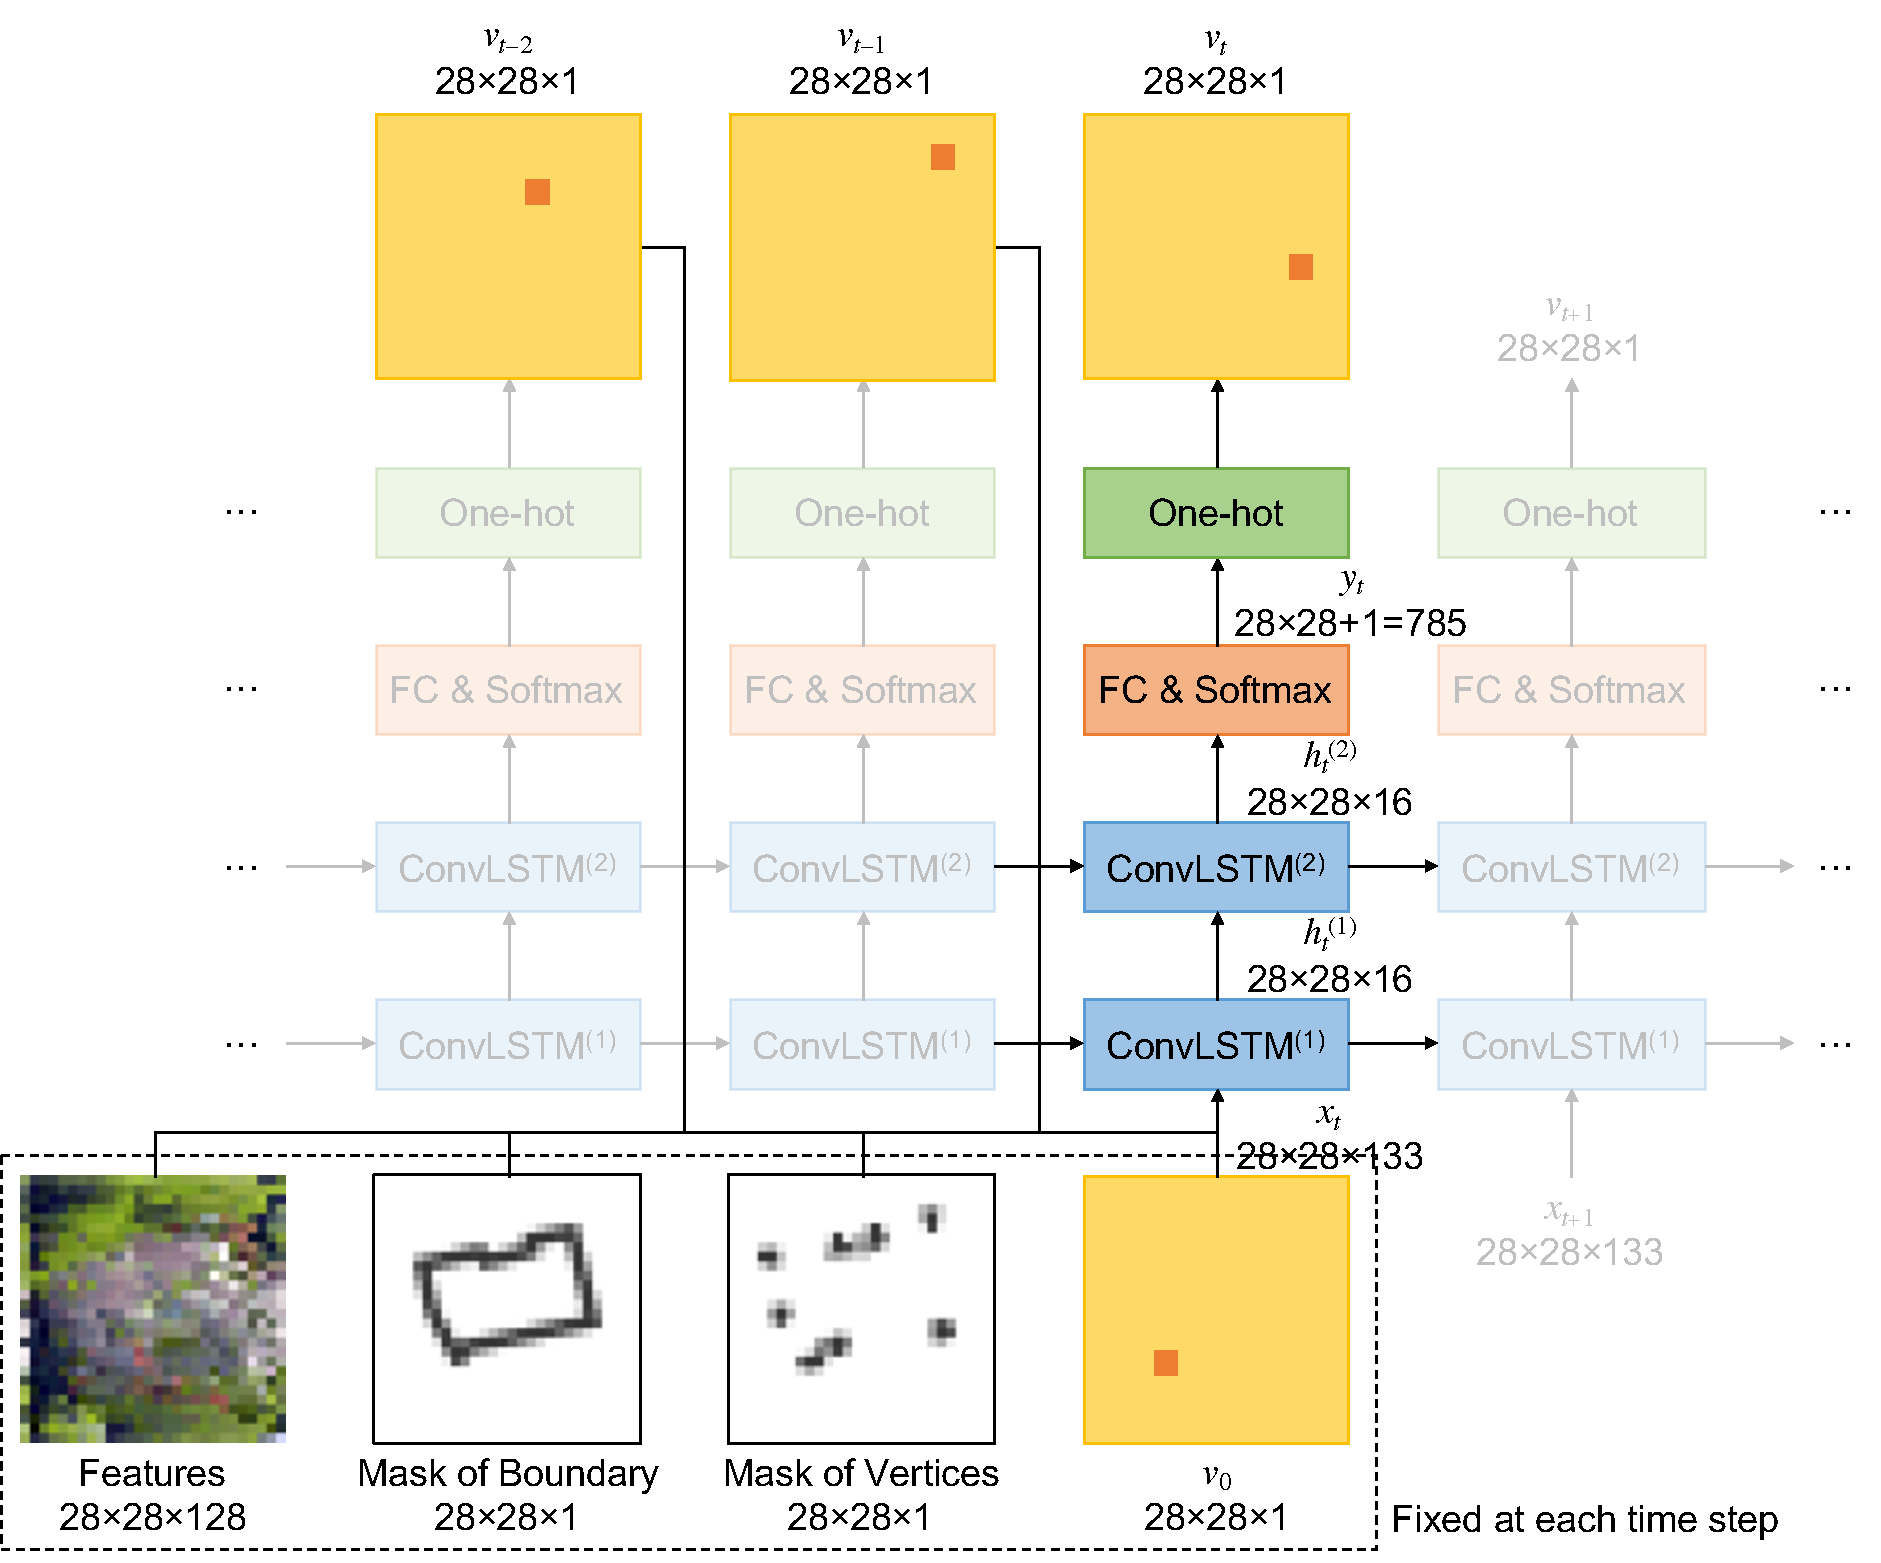
\includegraphics[width=\fig\textwidth]{3-05.pdf}
    \caption[Visualization for the time step of the RNN decoder]{Visualization for the time step of the RNN decoder. In this figure, the outputs of the end signal are omitted, and the configuration of the ConvLSTM cell is the same as what is used in the original PolygonRNN paper. Specifically, the paper sets the number of RNN layers to 2 and uses ConvLSTM cells with 3$\times$3 kernel size and 16 channels.}
    \label{fig:rnnconvlstm}
\end{figure}

\paragraph{Multilayer RNN}
PolygonRNN uses multilayer RNN with ConvLSTM cells. The connection between two neighboring layers can be described as follows, which means that the cell input of the current layer comes from the cell output of the previous layer.
\begin{equation}\label{eq:cellconnect}
	x_t^{(k)} = h_t^{(k-1)}, \forall k \in \{2,3,\ldots,n\},
\end{equation}
where $n$ is the number of RNN layers or ConvLSTM cells, $k$ in the superscript denotes the $k$-th layer. Recall that the initial cell input (i.e. the cell input of the first layer) at time step $t$ consists of the spatial information $f$ from CNN (including the masks of boundary and vertices), the two previous vertices $v_{t-1}$ and $v_{t-2}$, and starting vertex $v_0$, here it is formulated as follows.
\begin{equation}\label{eq:concat}
	x_t = x_t^{(1)} = v_{t-1} \oplus v_{t-2} \oplus v_0 \oplus f,
\end{equation}
where $\oplus$ denotes the concatenation operation in the dimension of channels. Thus, the equation \ref{eq:vnext} can be written as follows.
\begin{equation}\label{eq:probcomp}
	y_t = P(v_t \mid v_{t-1}, v_{t-2}) = \text{softmax}(W_y\text{vec}(h_t^{(n)})),
\end{equation}
where $W_y$ denotes the weights of the final fully connected layer, $\text{vec}(\cdot)$ denotes the vectorization function for a matrix. Figure \ref{fig:rnnconvlstm} shows the entire structure of the RNN part and highlights the process at time step $t$, using the same notation as the equations \ref{eq:cellconnect}, \ref{eq:concat} and \ref{eq:probcomp}.

Note that at each time step, the features, the masks of boundary and vertices as well as the one-hot encoding of starting vertex are fixed. Only $v_{t-1}$ and $v_{t-2}$ change over time.

\subsection{Loss Function}\label{losspoly}
The loss of PolygonRNN consists of two parts, loss of CNN and loss of RNN. The loss function of CNN part uses log loss, since the mask prediction is equivalent to binary classification for each pixel. We also notice that the non-boundary pixels or the non-vertex pixels occupy the majority, the loss function should be further weighted.
\begin{equation}
	L(M, M^*) = \sum_{i=1}^H\sum_{j=1}^W \left[w_p\mathbb{1}[M_{ij} = 1]\log{\frac{1}{M^*_{ij}}} + w_n\mathbb{1}[M_{ij} = 0]\log{\frac{1}{1-M^*_{ij}}} \right],
\end{equation}
\begin{equation}
	w_p = \frac{1}{2\sum_{i, j}\mathbb{1}[M_{ij} = 1]}, w_n = \frac{1}{2\sum_{i, j}\mathbb{1}[M_{ij} = 0]},
\end{equation}
where $L(M, M^*)$ denotes the loss function for the ground truth mask $M$ and predicted mask $M^*$, the subscript $i$ and $j$ denotes the $i$-th row and $j$-th column, $W$ and $H$ denote the width and height of mask, $\mathbb{1}[\cdot]$ denotes the indicator function, $w_p$ and $w_n$ denote the weights for positive and negative pixels, respectively. Thus, the loss of CNN part $L_{\text{CNN}}$ can be written as follows.
\begin{equation}
	L_{\text{CNN}} = L(M_b, M^*_b) + L(M_v, M^*_v),
\end{equation}
where subscript $b$ and $v$ denote masks of boundary and vertices, respectively. As for the loss of RNN, the loss function used is cross-entropy loss, because the polygon prediction is equivalent to multiclass classification at every time step. Thus, the loss of RNN part $L_{\text{RNN}}$ can be written as follows.
\begin{equation}
	L_{\text{RNN}} = \frac{1}{TK} \sum_{t=1}^T\sum_{k=1}^K\mathbb{1}[v_{t} = k]\log{\frac{1}{y_{tk}}},
\end{equation}
\begin{equation}
	y_{tk} = P(v_t = k \mid v_{t-1}, v_{t-2}),
\end{equation}
where $y_tk$ denotes the $k$-th component of $y_t$, i.e. the conditional probability of $v_t$ at the position $k$, given its two previous vertices, $T$ denotes the number of vertices in the polygon, $K$ denotes the number of possible assignments (positions) for vertex $v_t$ including the end signal. Here we do not consider the loss for the first vertex $v_0$, because it is randomly chosen from the polygon vertices when training. Finally, the total loss of PolygonRNN $L_{\text{PolygonRNN}}$ is defined as
\begin{equation}
	L_{\text{PolygonRNN}} = L_{\text{CNN}} + \gamma L_{\text{RNN}},
\end{equation}
where $\gamma$ is a self-defined weight.

\section{Feature Pyramid Network}\label{modfpn}
FPN \cite{fpn} is the core model for object detection in this project. Object detection problem is exactly multiple bounding boxes regression problem, which finds out multiple RoIs within an image. Subsection \ref{sglbboxreg} first illustrates problem of single bounding box regression. Subsection \ref{ancpro} introduces some basic concepts related to anchor, and subsection \ref{mulbboxreg} further illustrates multiple bounding boxes regression. Finally, subsection \ref{fpnbone} looks into the backbone of FPN, presents how feature pyramid is generated and how FPN can tackle the multi-scale detection problem.

\subsection{Single Bounding Box Regression}\label{sglbboxreg}
Single bounding box regression can be used for such a scenario, where the image contains only one object. Generally, a bounding box can be uniquely determined by four parameters, either box center and box size, denoting $(x, y)$ and $(w, h)$ or the coordinates of the upper left and lower right corners of the box, denoting $(l, u)$ and $(r, d)$. They have following relationships.
\begin{equation}
	\left[\begin{array}{c}
		x\\y\\w\\h
	\end{array}\right]=\frac{1}{2}\left[\begin{array}{cccc}
		1 & 0 & 1 & 0 \\
		0 & 1 & 0 & 1 \\
		-2 & 0 & 2 & 0 \\
		0 & -2 & 0 & 2
	\end{array}\right]\left[\begin{array}{c}
		l\\u\\r\\d
	\end{array}\right],
\end{equation}
\begin{equation}
	\left[\begin{array}{c}
		l\\u\\r\\d
	\end{array}\right]=\frac{1}{2}\left[\begin{array}{cccc}
		2 & 0 & -1 & 0 \\
		0 & 2 & 0 & -1 \\
		2 & 0 & 1 & 0 \\
		0 & 2 & 0 & 1
	\end{array}\right]\left[\begin{array}{c}
		x\\y\\w\\h
	\end{array}\right].
\end{equation}
Therefore, we can regard the problem of finding out object's bounding box as a parameter regression problem. With the image as input, either set of the four parameters, $(x, y, w, h)$ or $(l, u, r, d)$, can be selected as the target for the regression. Figure \ref{fig:sglbboxreg} shows the architecture of the network for single bounding box regression, using box center and size as outputs.

\begin{figure}[!h]
	\centering
	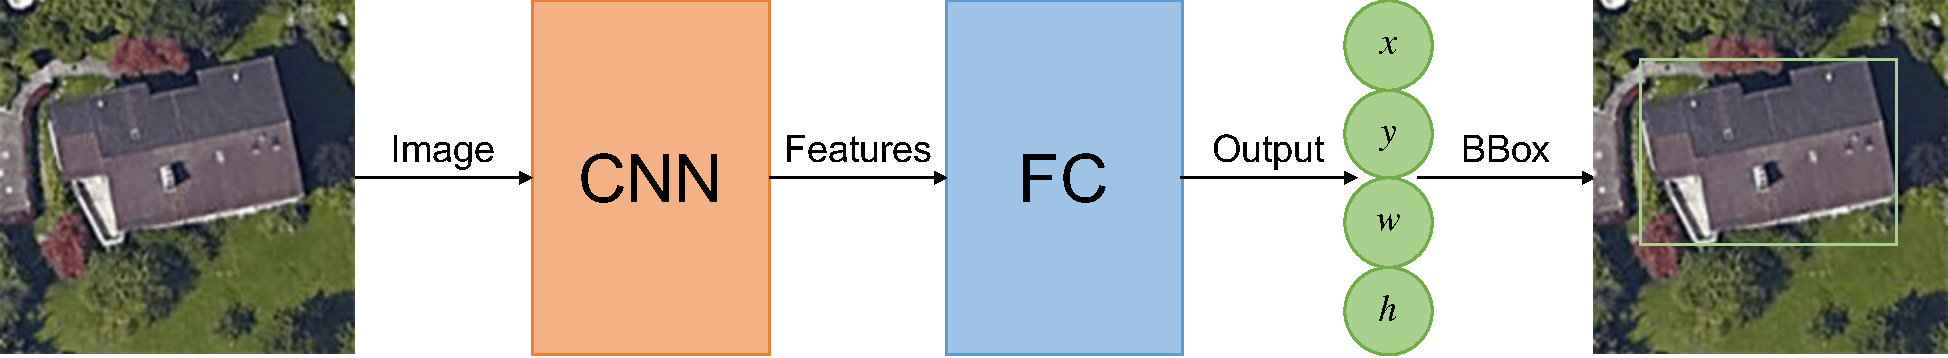
\includegraphics[width=\fig\textwidth]{3-06.pdf}
    \caption[Simplified structure of the network for single bounding box regression]{Simplified structure of the network for single bounding box regression. In this figure, the output of FC layer refers to the center and size of the bounding box.}
    \label{fig:sglbboxreg}
\end{figure}

In practice, usually the normalized parameters of box center and size rather than the coordinates of two corners are used as training targets. As for the normalization functions, please see subsection \ref{mulbboxreg} for more details.

\subsection{Anchor and Its Properties}\label{ancpro}
Anchor is a basic concept in multiple bounding boxes regression. The following paragraphs introduce the idea of anchor and its properties in detail.

\paragraph{Anchor}
An anchor refers to an artificially specified bounding box in the original image, regardless of the number of RoIs or where these RoIs locate. An arbitrary rectangular area in the image can be an anchor. For an image with width $w$ and height $h$, the total number of possible anchors $n$ can be calculated as
\begin{equation}\label{eq:numanchor}
	n = \frac{1}{4}w(w+1)h(h+1).
\end{equation}
Thus, even for a very small image patch with size 224$\times$224, $n$ is already very large, reaching 635.04 million. Figure \ref{fig:eganchor} illustrates some examples of anchors in an image with multiple RoIs.

\begin{figure}[!h]
	\centering
	\subbottom[]
		{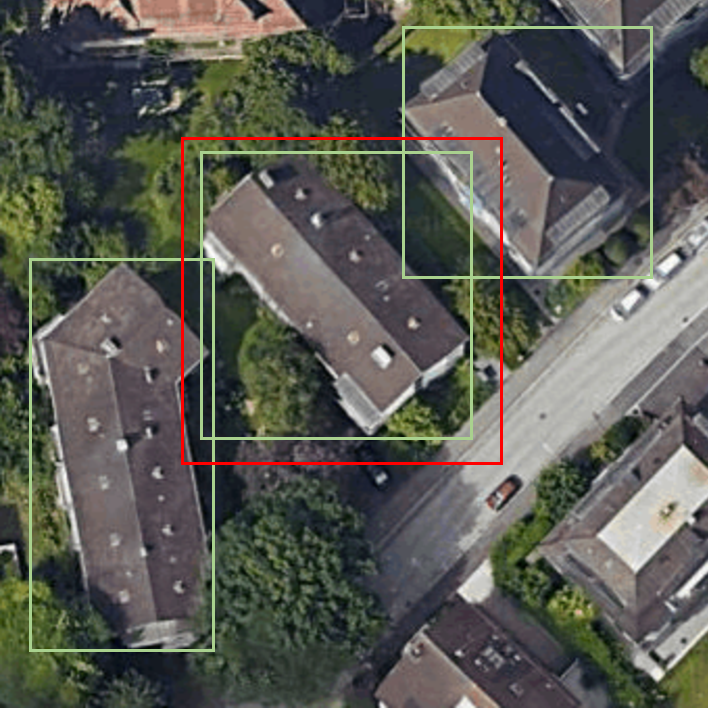
\includegraphics[width=\figfigfigfig\textwidth]{3-07-0.pdf}}
	\subbottom[]
		{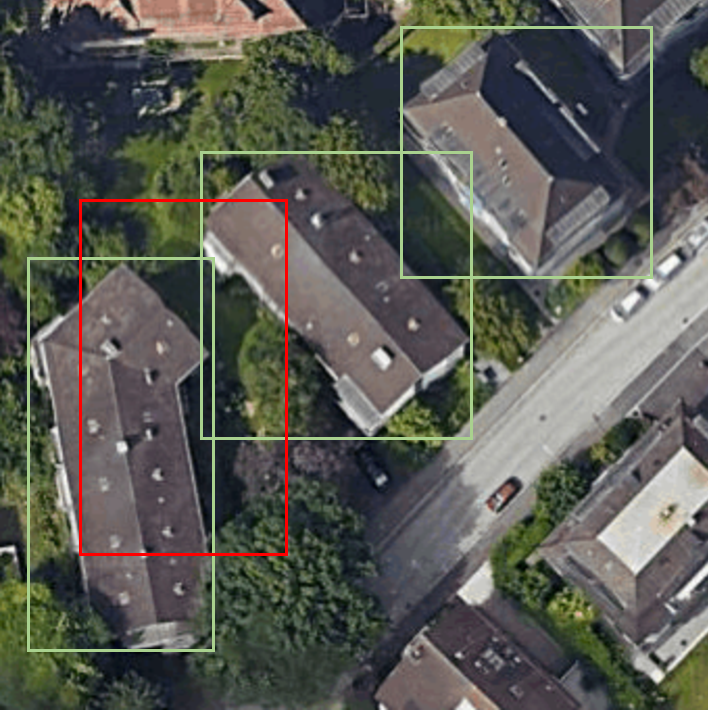
\includegraphics[width=\figfigfigfig\textwidth]{3-07-1.pdf}}
	\subbottom[]
		{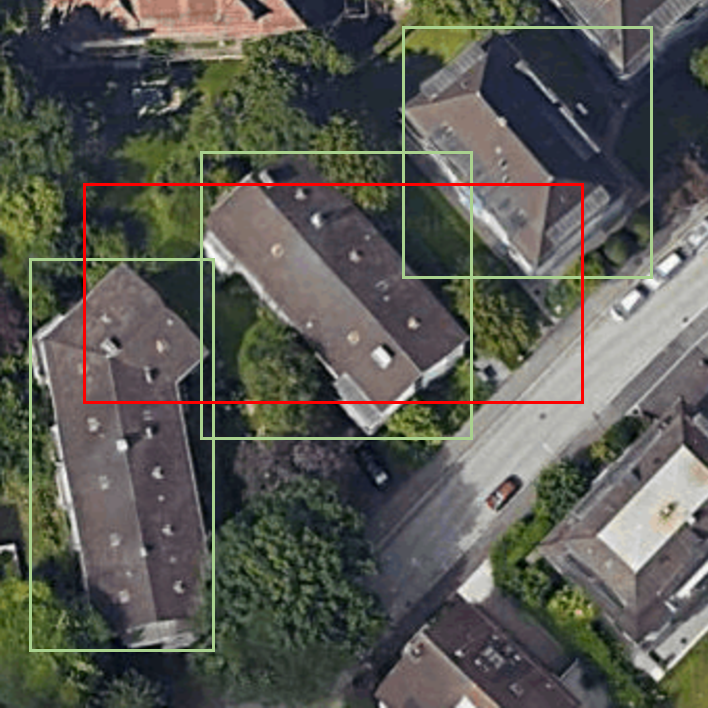
\includegraphics[width=\figfigfigfig\textwidth]{3-07-2.pdf}}
	\subbottom[]
		{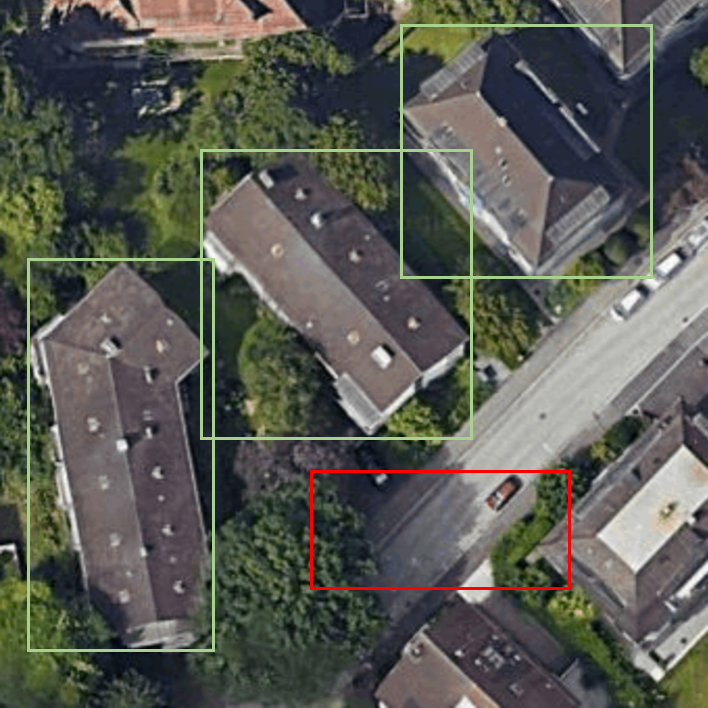
\includegraphics[width=\figfigfigfig\textwidth]{3-07-3.pdf}}
    \caption[Example anchors in image with multiple RoIs]{Example anchors in image  with multiple RoIs. (a)--(d) show four possible anchors in an image with  with multiple RoIs, with each showing one anchor. The red and light green rectangles refer to anchors and ground truth bounding boxes respectively.}
	\label{fig:eganchor}
\end{figure}

\paragraph{IoU Score}
Usually IoU (Intersection over Union) score is used to evaluate the distance between an anchor and a ground truth bounding box. The following equation shows its calculation. Note that the score's computation is irrelevant to the actual image content in either anchor or the ground truth bounding box.
\begin{equation}
	s = \frac{\lvert A \cap T \rvert}{\lvert A \cup T \rvert} \in [0, 1],
\end{equation}
where $s$ denotes the IoU score, $\lvert \cdot \rvert$ denotes the size of a set, $A$ and $T$ refer to the sets of pixels covered by the anchor and the ground truth bounding box respectively. $s = 1$ means that the anchor and the ground truth bounding box overlap perfectly. Figure \ref{fig:egiou} shows the coverage level under different IoU scores.

\begin{figure}[!h]
	\centering
	\subbottom[IoU = 0]
		{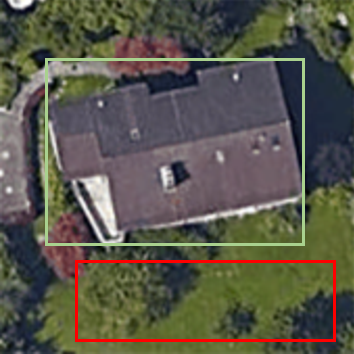
\includegraphics[width=\figfigfigfig\textwidth]{3-08-0.pdf}}
	\subbottom[IoU = 0.3]
		{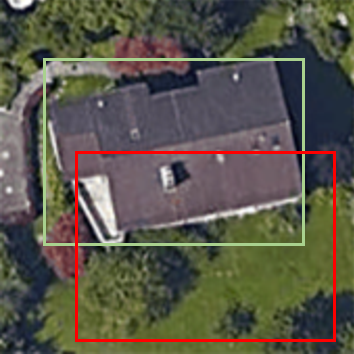
\includegraphics[width=\figfigfigfig\textwidth]{3-08-1.pdf}}
	\subbottom[IoU = 0.7]
		{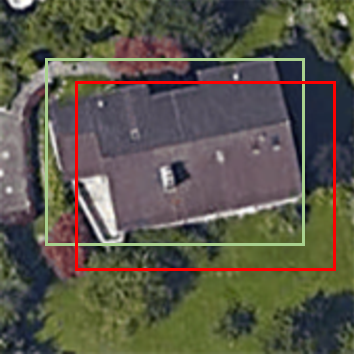
\includegraphics[width=\figfigfigfig\textwidth]{3-08-2.pdf}}
	\subbottom[IoU = 1]
		{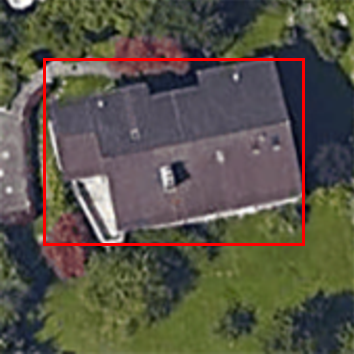
\includegraphics[width=\figfigfigfig\textwidth]{3-08-3.pdf}}
    \caption[Coverage level of anchor and ground truth bounding box under different IoU scores]{Coverage level of anchor and ground truth bounding box under different IoU scores.}
	\label{fig:egiou}
\end{figure}

\paragraph{Anchor Polarity}
Typically, there are several buildings in an aerial image, thus multiple RoIs exist. Based on the IoU scores of an anchor with these ground truth bounding boxes, we can make a judgment on the polarity of this anchor, which is defined as follows.
\begin{equation}
	s_i = \max_{j} \text{IoU}(a_i, b_j),
\end{equation}
\begin{equation}
\begin{aligned}
	p_i = \begin{cases}
		1, & s_i > t_h, \\
		0, & t_l \leqslant s_i \leqslant t_h,\\
		-1, & s_i < t_l,
	\end{cases}
\end{aligned}
\end{equation}
where $a_i$ and $b_j$ denote the $i$-th anchor and $j$-th ground truth bounding box, $s_i$ denotes the highest IoU score that $a_i$ can get, i.e. the IoU score of $a_i$ and its ``closest" ground truth bounding box, $p_i$ denotes the polarity of $a_i$, $t_l$ and $t_h$ denote two manually set thresholds for polarity judgment, and typically, $t_h = 0.7$, $t_l = 0.3$. An anchor is labeled as positive, natural or negative in case of $p_i = 1$, $p_i = 0$ or $p_i = -1$, respectively. Figure \ref{fig:eganchor} also shows anchors with different polarities using typical thresholds.

\subsection{Multiple Bounding Boxes Regression}\label{mulbboxreg}
Multiple bounding boxes regression can be very different from the single one. Since the number of RoIs is unknown, if we still directly use the idea of parameters regression as what we do in case of the single bounding box, then the number of nodes of the FC output layer will not be fixed. In addition, the RoIs in the image usually reflect the local information, thus we cannot directly use all global features obtained by CNN, either.

\paragraph{Anchor Assignment}
The basic idea for multiple bounding boxes regression is to regress them on positive anchors. Specifically, each RoI is regressed on the anchors which are assigned to it. There are two rules for the assignment: (1) each ground truth bounding box should have at least one anchor (either positive, natural or negative) assigned to it; (2) each positive anchor should be assigned to its ``closest" ground truth bounding box. For those non-positive anchors that have assignments, we also treat them as positive anchors. For details of the matching algorithm, please refer to section \ref{app:assignanchor}.

\paragraph{Classification and Regression on Anchors}
As a matter of fact, the single bounding box regression can be also regarded as regression on the anchor. Here the anchor is exactly the whole image. Similar to this, we can simply increase the number of nodes in the FC output layer (see figure \ref{fig:sglbboxreg}) according to the number of anchors. Generally, each anchor requires 6 output nodes, 2 for binary classification and 4 for parameters regression. Specifically, 2 classification nodes output the logits, denoting $l_p$ and $l_n$, indicating how close the anchor is to an RoI. Thus, the predicted probability of an anchor referring to an RoI $p^*$ can be calculated as follows, using softmax function.
\begin{equation}
	p^* = \frac{e^{l_p}}{e^{l_p} + e^{l_n}}, 1 - p^* = \frac{e^{l_n}}{e^{l_p} + e^{l_n}}.
\end{equation}
The rest 4 regression nodes output the information of the refined box, for recovering the corresponding RoI. Suppose we have a fixed positive anchor, which is assigned to a ground truth bounding box. The parameters of refined (or normalized) box are used for regression target, which can be calculated as
\begin{equation}
	r_x = \frac{x_g - x_a}{w_a}, r_y = \frac{y_g - y_a}{h_a}, r_w = \log\frac{w_g}{w_a}, r_h = \log\frac{h_g}{h_a},
\end{equation}
where $(x_a, y_a, w_a, h_a)$ and $(x_g, y_g, w_g, h_g)$ denotes the four parameters of the anchor and the ground truth bounding box respectively, $(r_x, r_y, r_w, r_h)$ denotes the refined parameters for regression target. The following equations define the recovery phase.
\begin{equation}
	x_g^* = x_a + r_x^*w_a, y_g^* = h_a + r_y^*h_a, w_g^* = w_ae^{r_w^*}, h_g^* = h_ae^{r_h^*},
\end{equation}
where $(r_x^*, r_y^*, r_w^*, r_h^*)$ and $(x_g^*, y_g^*, w_g^*, h_g^*)$ denote the predicted refinement parameters and the parameters of the final predicted bounding box respectively. The reason why the refined parameters are used for training, instead of original box, is that the former one eliminates the shape and location information of original box, hence it is more suitable for calculating the loss.

\begin{figure}[!h]
	\centering
	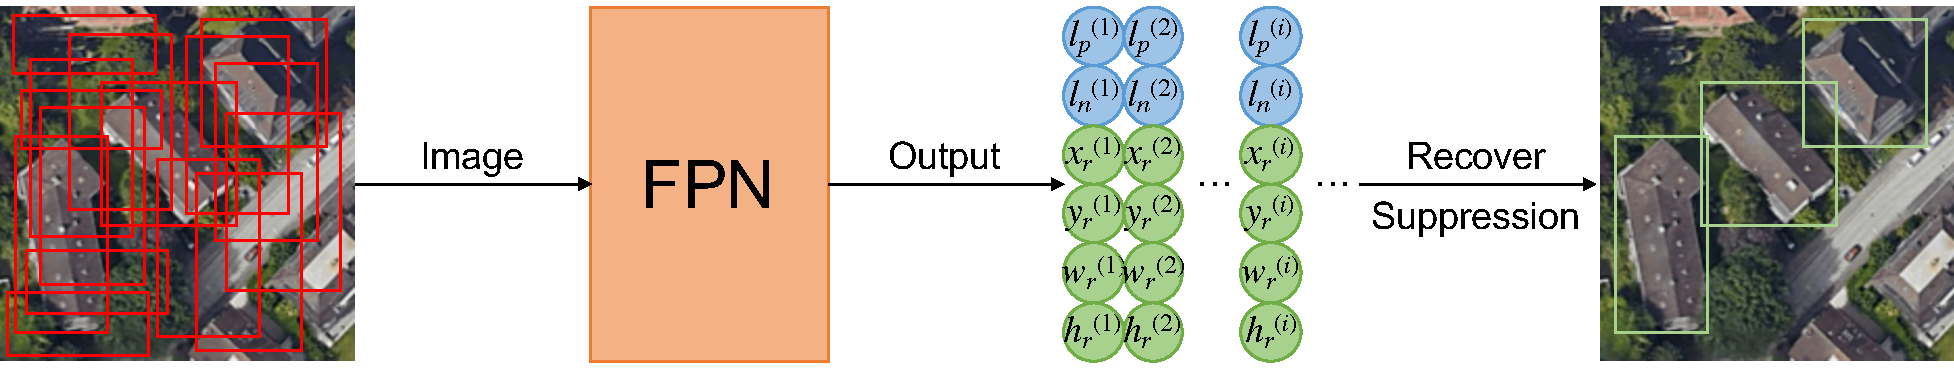
\includegraphics[width=\fig\textwidth]{3-09.pdf}
    \caption[Smooth $L_1$ loss function]{Smooth $L_1$ loss function.}
    \label{fig:l1loss}
\end{figure}

\paragraph{Loss}
As for training, only positive and negative anchors are used, where classification uses both and regression uses positive anchors only. The loss function used for classification is log loss, which is described as follows (for a single anchor).
\begin{equation}
	L_c = \mathbb{1}[p = 1]\log{\frac{1}{p^*}} + \mathbb{1}[p = -1]\log{\frac{1}{1-p^*}},
\end{equation}
where $L_c$ is the classification loss, $p$ is the polarity of the anchor, $p^*$ is the predicted probability, $\mathbb{1}[\cdot]$ is the indicator function. Additionally, the loss used for regression is the smooth $L_1$ loss, which is described as
\begin{equation}
\begin{aligned}
	f(x) = \begin{cases}
		\dfrac{1}{2}x^2, & \lvert x \rvert < 1, \\
		\lvert x \rvert - \dfrac{1}{2}, & \lvert x \rvert \geqslant 1,
	\end{cases}
\end{aligned}
\end{equation}
\begin{figure}[!h]
	\centering
	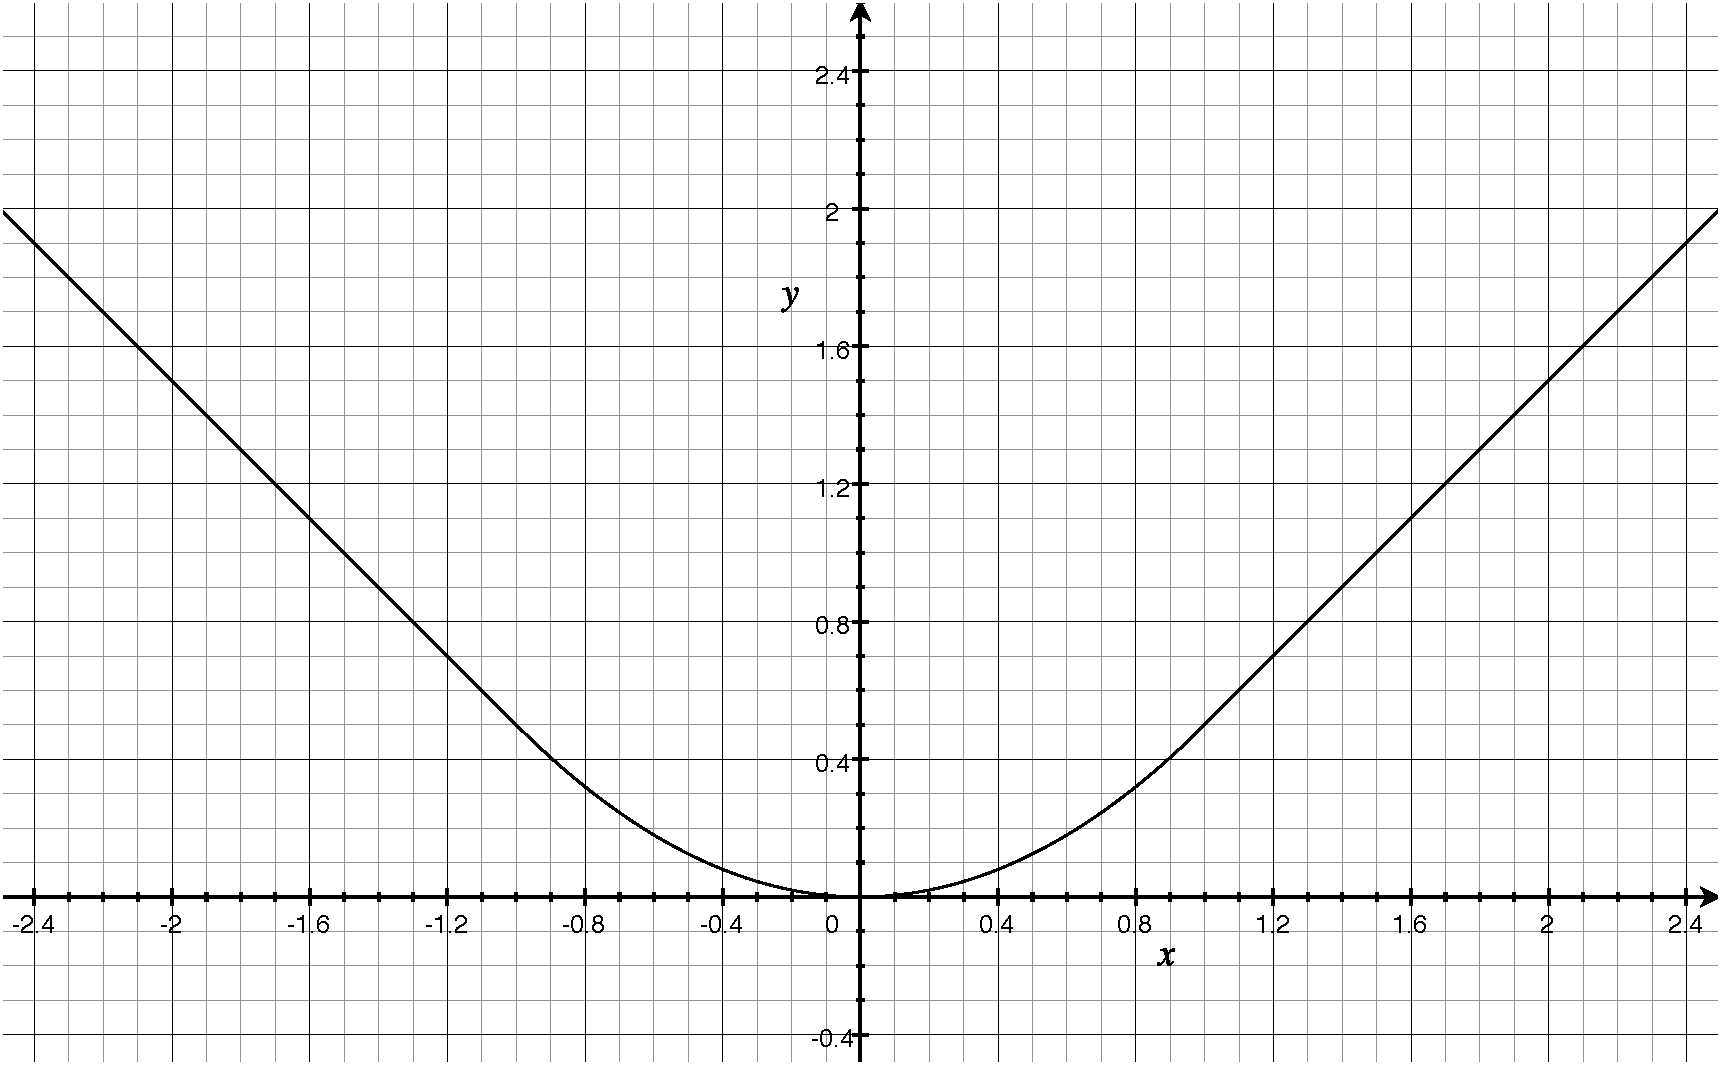
\includegraphics[width=\figfi\textwidth]{3-10.pdf}
    \caption[Smooth $L_1$ loss function]{Smooth $L_1$ loss function.}
    \label{fig:l1loss}
\end{figure}
\begin{equation}
	L_r = f(x_g^* - x_g) + f(y_g^* - y_g) + f(w_g^* - w_g) + f(h_g^* - h_g),
\end{equation}
where $L_r$ is the regression loss. The total loss of FPN $L_{\text{FPN}}$ is defined as
\begin{equation}
	L_{\text{FPN}} = \sum_{i}^{} L_c^{(i)} + \lambda\sum_{i}^{}\mathbb{1}[p_i = 1]L_r^{(i)},
\end{equation}
where the superscript $i$ denotes the $i$-th anchor, $\lambda$ denotes a self-defined parameter when training.

\subsection{Feature Pyramid and Backbone}\label{fpnbone}

From equation \ref{eq:numanchor} we know that even a small image can have a huge number of possible anchors. However, it is impossible to involve all anchors in the training phase, since the output layer would have too many nodes and the number of parameters in the network would explode. Thus, how to select appropriate number of anchors in the original image remains a problem. But there is no doubt that the selected anchors should not ``miss" any ground truth bounding box (i.e. should ``cover" the ground truth bounding boxes as much as possible). Under this guideline, selected anchors should have different kinds of shapes, in different scales and evenly distributed in the image.

\paragraph{Anchor Selection in RPN}
In fact, in RPN from Faster R-CNN \cite{fasterrcnn}, there is a simple way to select anchors. For each entry of the convoluted feature map (or for each pixel of the original image with corresponding stride), we generate $k$ different shapes of anchors with different scales, which is shown in figure \ref{fig:ancsel}. For example, if we select anchors from an image with size 320$\times$320, choosing stride 8$\times$8 (corresponding to the feature map with size 40$\times$40), 3 different shapes (1:1, $\frac{\sqrt{2}}{2}$:$\sqrt{2}$, $\sqrt{2}$:$\frac{\sqrt{2}}{2}$) and 4 scales (16, 32, 64, 128), then we have $40^2\times3\times4=19200$ anchors.

\begin{figure}[!h]
	\centering
	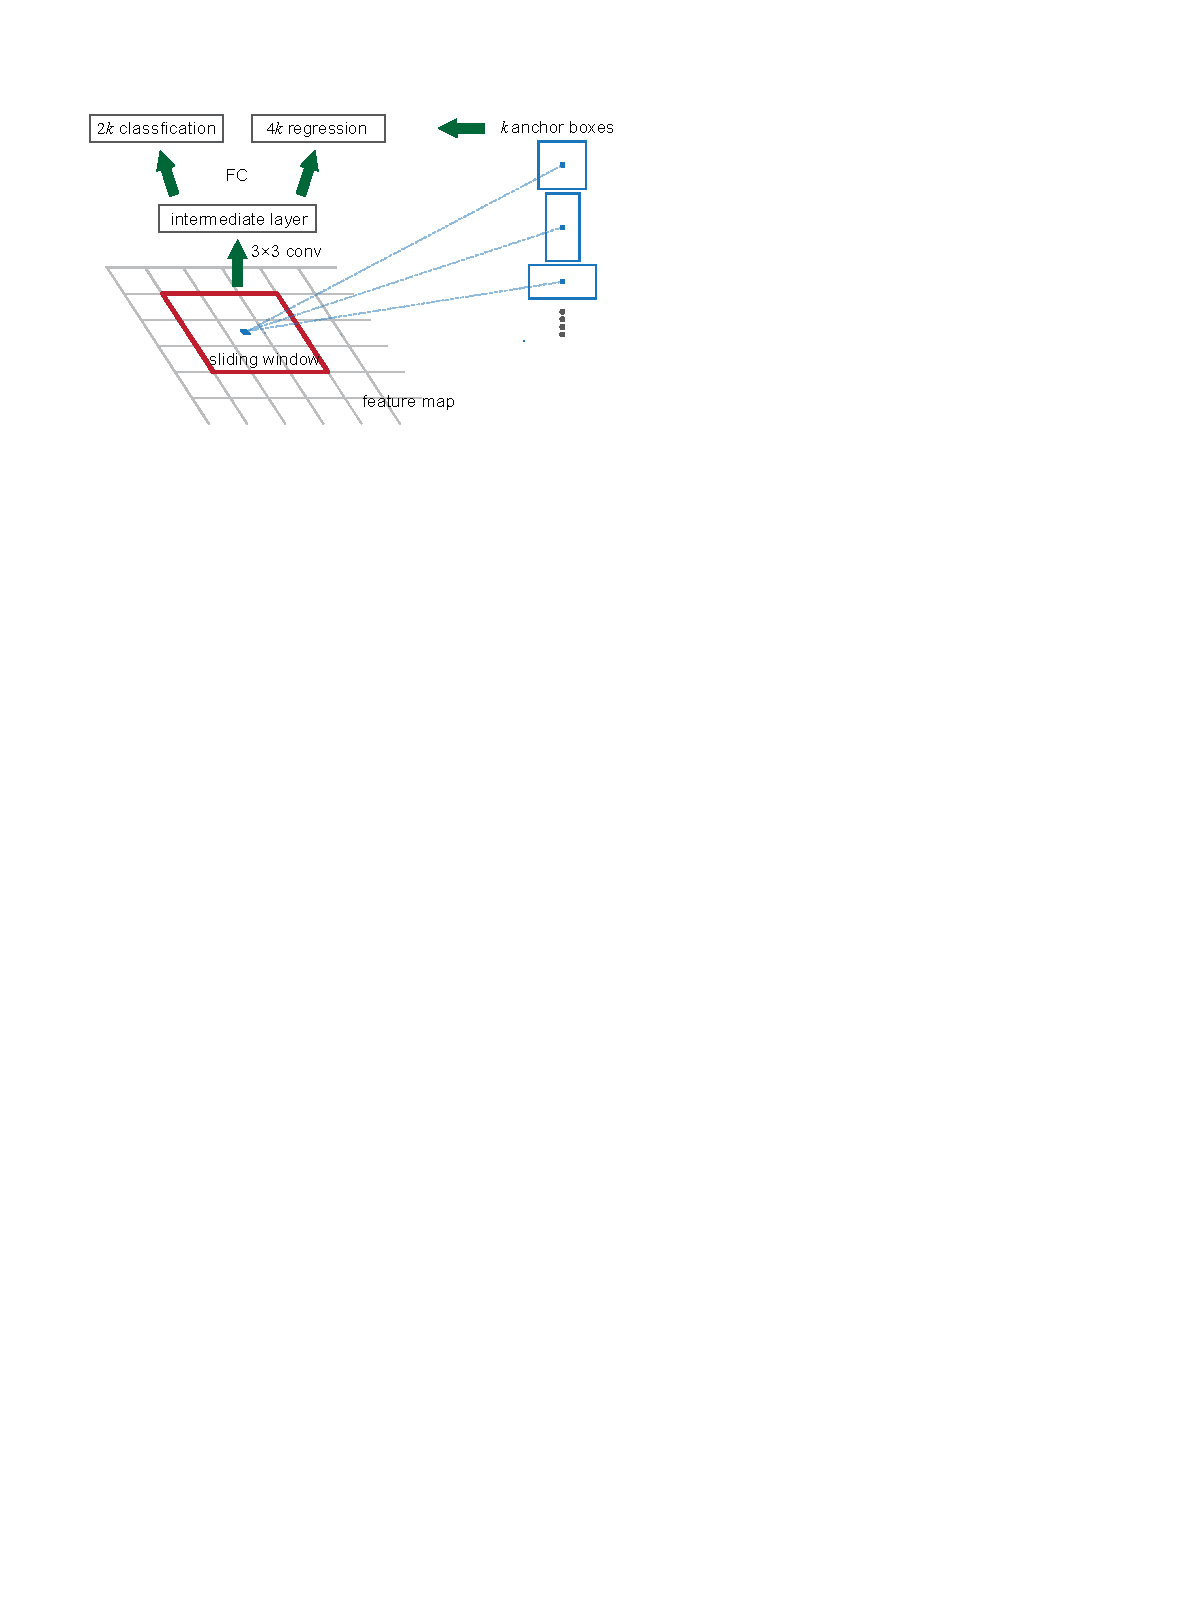
\includegraphics[width=\figfi\textwidth]{3-11.pdf}
    \caption[Anchor selection and regression part of RPN/FPN]{Anchor selection and regression part of RPN/FPN. Image copyright owned by \cite{fasterrcnn}.}
    \label{fig:ancsel}
\end{figure}

But this method produces two problems: (1) Large anchors are very close to each other, resulting in redundancy; (2) The stride may be too large for small anchors, thus a typically small ground truth bounding box, which are sandwiched between two small anchors, is very likely to be ``missed". Actually, the second one is the reason why RPN cannot well detect small objects. However, both problems are tackled with the introduction of feature pyramid.

\paragraph{Anchor Selection in FPN}
Feature pyramid is a basic component in recognition systems for detecting objects. It actually refers to semantic feature maps at different scales. FPN exploits the inherent multi-scale, pyramidal hierarchy of deep convolutional networks to construct feature pyramids. The network uses a top-down architecture with lateral connections, which is developed for constructing an in-network feature pyramid from a single-scale input. Figure \ref{fig:fpn} shows its architecture.

\begin{figure}[!h]
	\centering
	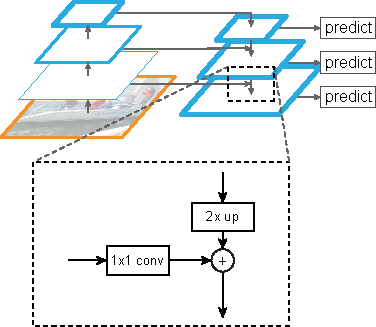
\includegraphics[width=\figfi\textwidth]{3-12.pdf}
    \caption[Structure of Feature Pyramid Network]{Structure of Feature Pyramid Network. The upper left part is the general convolutional process. The upper right part shows the feature pyramid. The lower part shows the lateral connections in detail.}
    \label{fig:fpn}
\end{figure}

The relationship between the feature pyramid and anchors is that each level of the feature pyramid corresponds to single scale of anchors, which can be seen in figure \ref{fig:ancdifflay}. In general, we have
\begin{equation}
	S_i = 2^{i-1}S_1, i \in \{1,2,\ldots\},
\end{equation}
where $S_1$ denotes the smallest anchor scale (typically around 20, e.g. 16--24), $S_i$ denotes the anchor scale corresponding to the feature map with $2^{-i}$ resolution. For example, for an image with size 320$\times$320, if the smallest anchor scale is set to be 16, the anchor scale for the feature map with resolution 40$\times$40 would be 128.

\begin{figure}[!h]
	\centering
	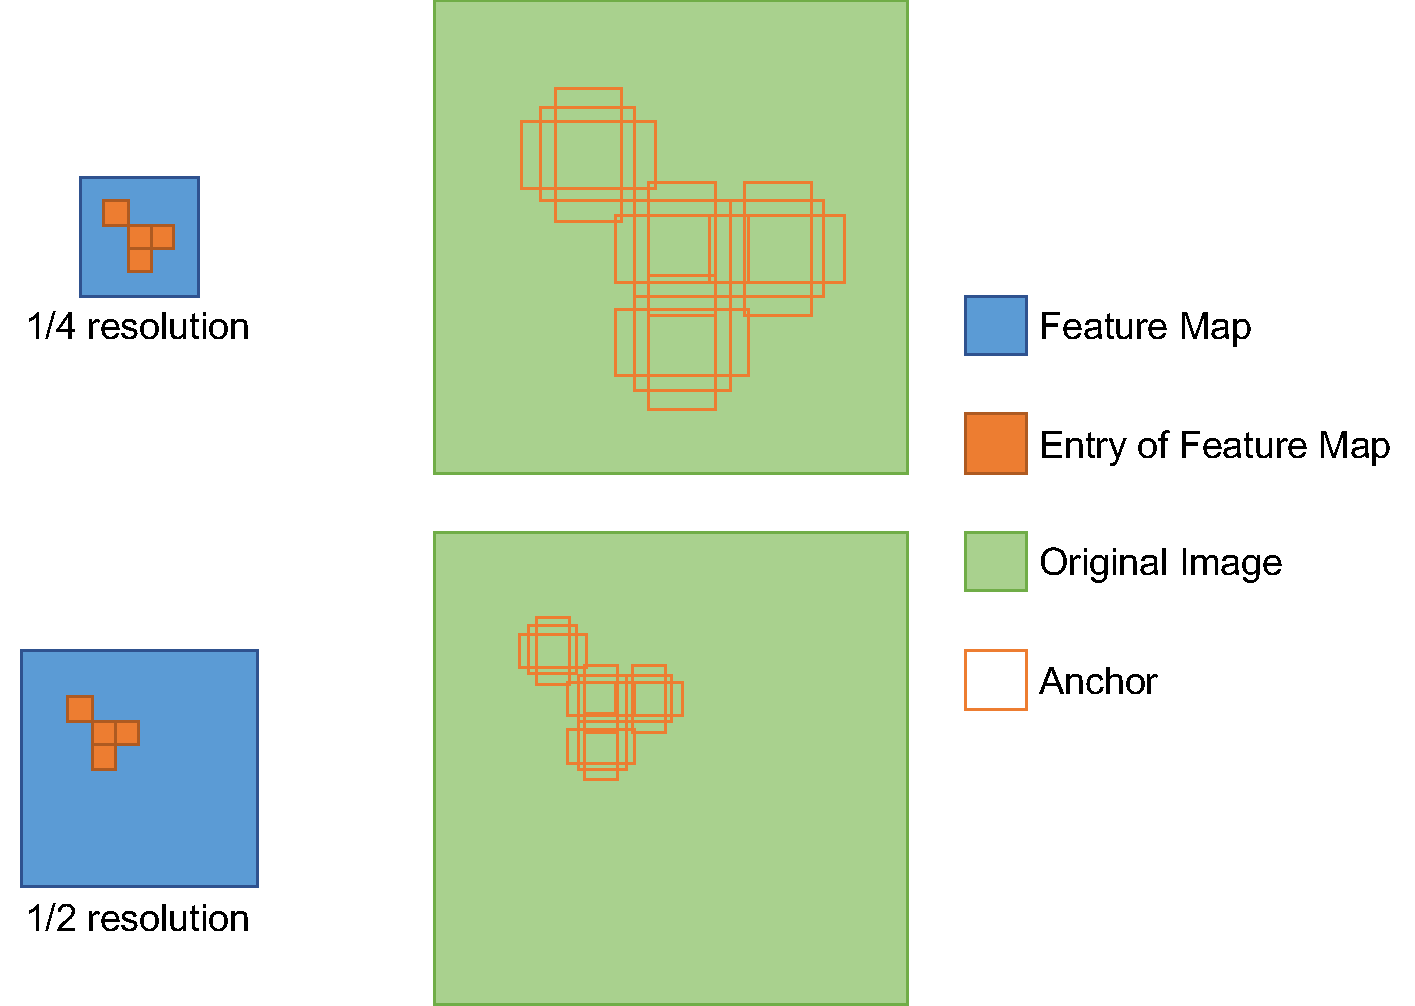
\includegraphics[width=\figfi\textwidth]{3-13.pdf}
    \caption[Generation of anchors from different layers of feature pyramid]{Generation of anchors from different layers of feature pyramid.}
    \label{fig:ancdifflay}
\end{figure}

Therefore, in FPN, the feature map with larger resolution corresponds to smaller anchor scale, with smaller stride with regard to the original image. Similarly, the feature map with smaller resolution corresponds to larger anchor scale, with larger stride with regard to the original image. This is the core reason why the problems mentioned around figure \ref{fig:ancsel} can be addressed. On the other hand, the total number of anchors $n_l$ has an upper bound $\Theta(wh)$, which can be derived from
\begin{equation}
	n_l = \sum_{i=1}^{l}\frac{w}{2^i}\frac{h}{2^i}k=whk\sum_{i=1}^{l}4^{-i}=\frac{1}{3}whk(1-4^{-l}) < \frac{1}{3}whk,
\end{equation}
where the subscript $l$ denotes the number of layers (or feature maps) in the feature pyramid, i.e. the depth of feature pyramid, $w$ and $h$ denotes the image width and height, $k$ denotes the number of manually designed anchor shapes. Compared with equation \ref{eq:numanchor}, the total number of anchors is reduced by two orders of magnitude.

\paragraph{Backbone of FPN}
The upper left part of figure \ref{fig:fpn} is so-called backbone of FPN, which is exactly a general CNN. In Mask R-CNN \cite{maskrcnn}, the backbone used for feature extraction is ResNet-101 \cite{resnet}, which can give excellent gains in both accuracy and speed. However, in our project, VGG-16 \cite{vgg16} is chosen as the backbone of FPN, because we want FPN and PolygonRNN share the same VGG-16. For more details about the shared VGG-16, please refer to subsection \ref{hybmod}.

Figure \ref{fig:fpnvgg} shows the architecture of FPN with VGG-16 backbone used in our project for feature pyramid extraction. Actually, the lateral connections are not limited to a fixed method, which means that each layer of VGG-16 can be lead out using a reasonable connection. Here we use 4-layer feature pyramid, and features are taken from layers \lstinline{conv3_3}, \lstinline{conv4_3} and \lstinline{conv5_3}, respectively. For the network to make further prediction of refined box parameters, it is the same as what is shown in figure \ref{fig:ancsel}.

\begin{figure}[!h]
	\centering
	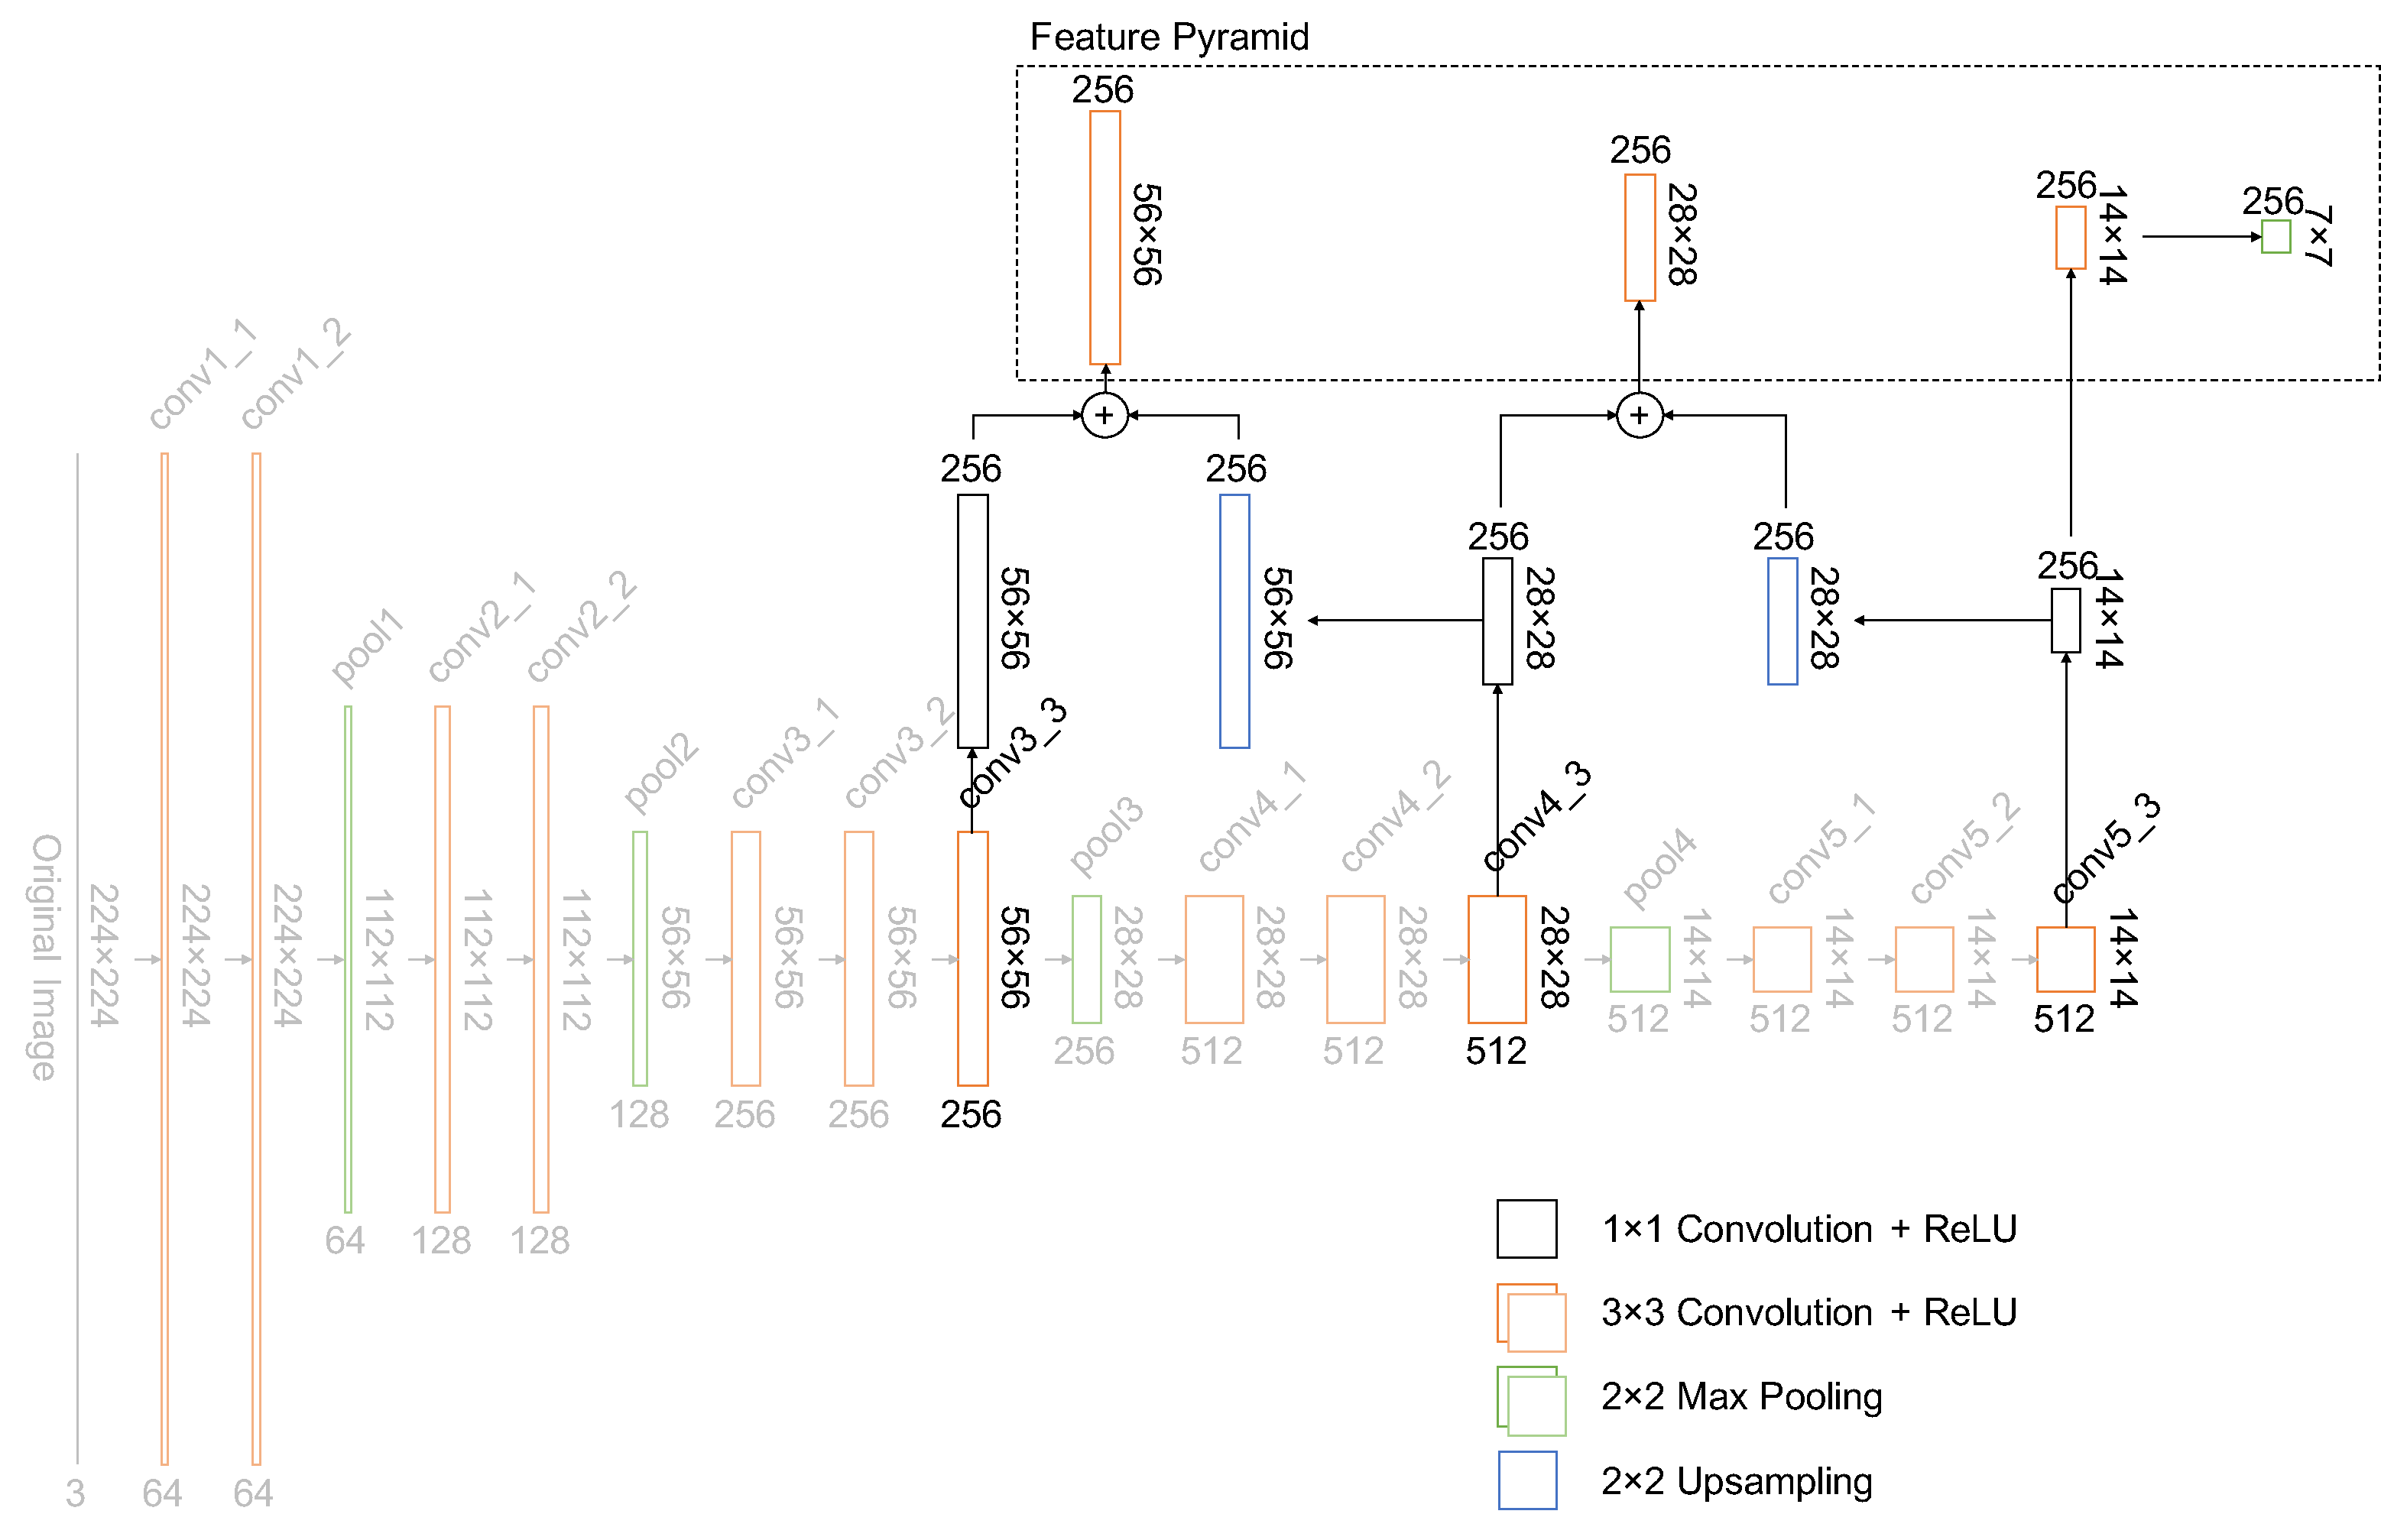
\includegraphics[width=\fig\textwidth]{3-14.pdf}
    \caption[FPN with VGG-16 backbone.]{FPN with VGG-16 backbone.}
    \label{fig:fpnvgg}
\end{figure}

\section{\modelnameshort}\label{modmer}

In this section, the final model, \modelnameshort\ (\modelnamelong), is derived and introduced in detail. Here we propose 3 possible versions, denoting two-step version, hybrid version and hybrid version with RoIAlign, which are described in subsection \ref{stpmod}, \ref{hybmod} and \ref{algmod}, respectively.

\subsection{Two-step Version}\label{stpmod}

The two-step version is very natural and easy to think of. In the first step, RPN is used to get the RoIs from the aerial image and each RoI contains a building. In the second step, PolygonRNN is used to get the geometrical shape. Thus, our problem is solved after these two steps. Figure \ref{fig:stpmod} shows its pipeline.

\begin{figure}[!h]
	\centering
	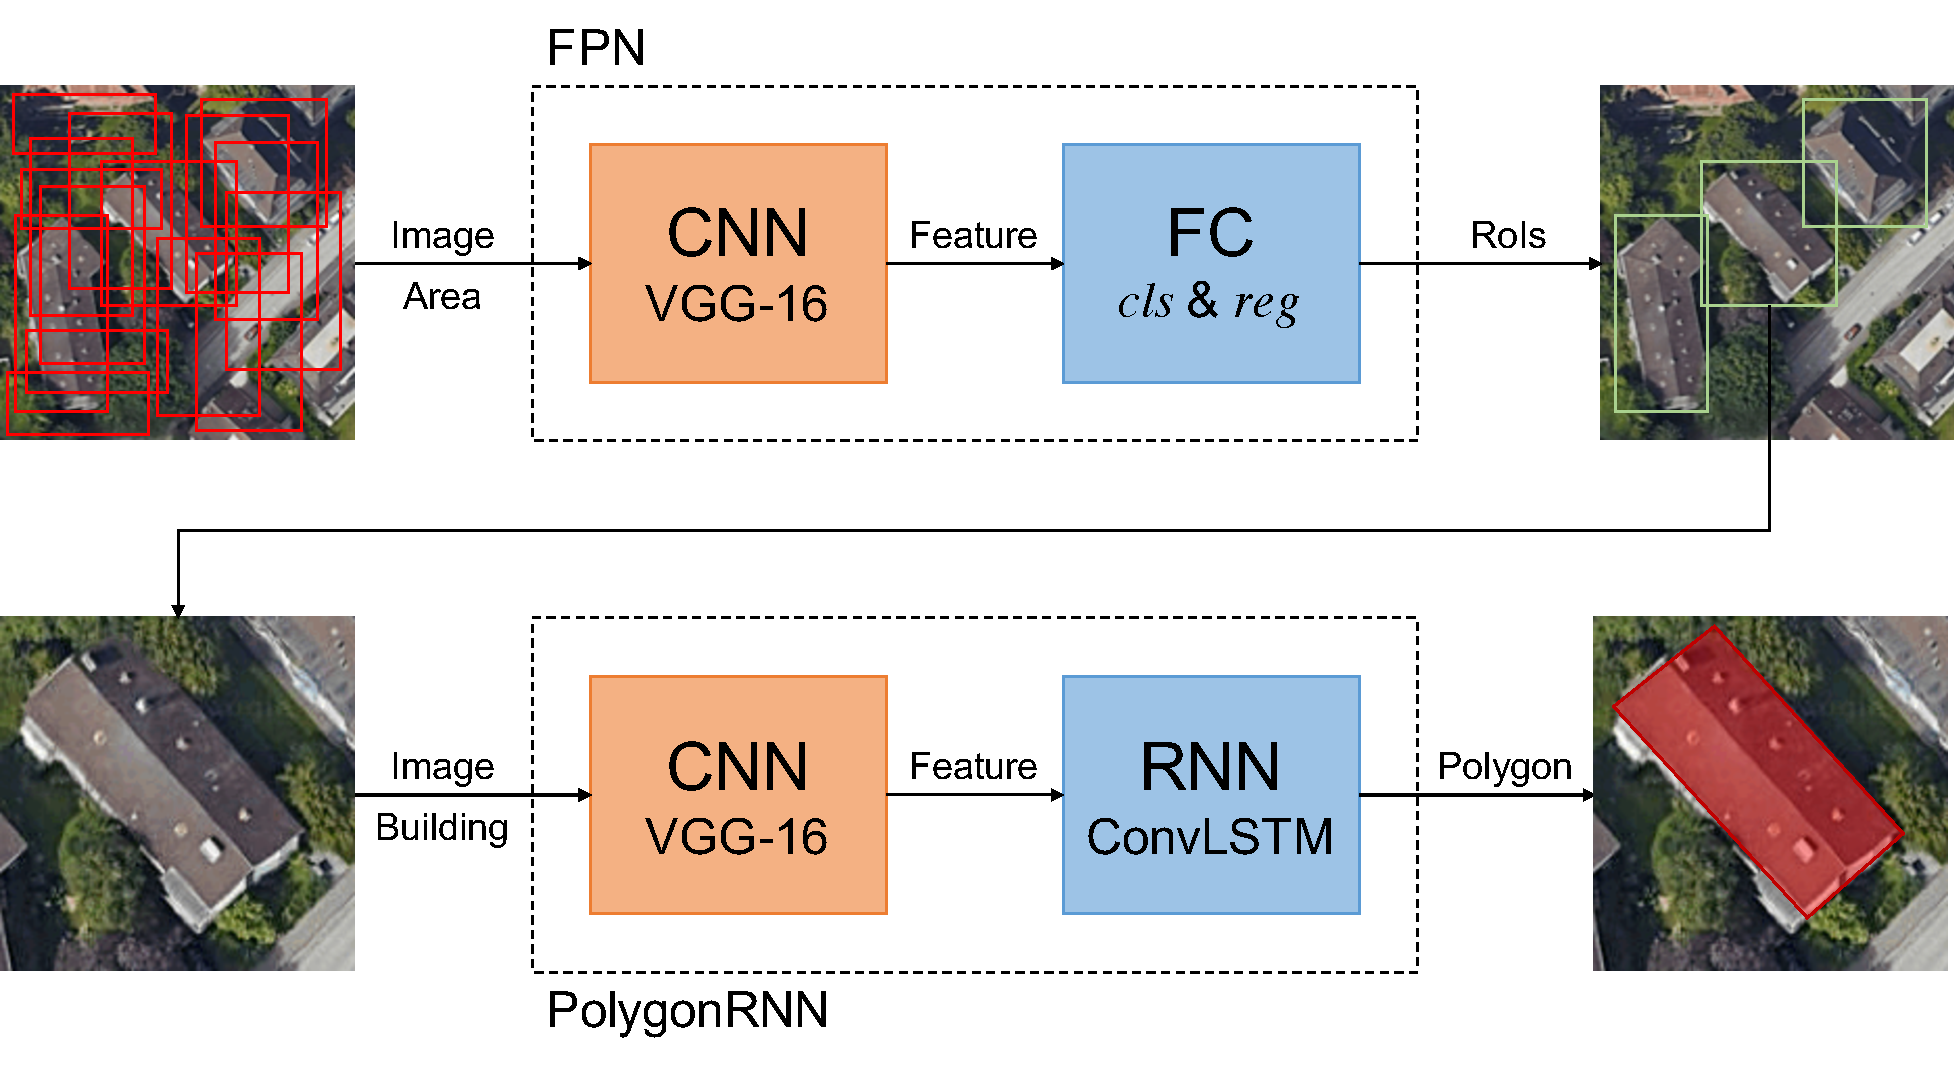
\includegraphics[width=\fig\textwidth]{3-15.pdf}
    \caption[\modelnameshort\ , two-step version]{\modelnameshort\ , two-step version.}
    \label{fig:stpmod}
\end{figure}

From the figure \ref{fig:stpmod} we can see that RPN and PolygonRNN are completely separate in this version. Therefore, during the training phase, we can train the two models separately and integrate them when making prediction (also possible to train together).

\subsection{Hybrid Version}\label{hybmod}
Note that in figure \ref{fig:stpmod}, either when the aerial image is taken as input by FPN or when the building image is taken as input by PolygonRNN, they both pass CNN first, and their CNNs both adopt VGG-16. In fact, regardless of the whole model of FPN or PolygonRNN, focusing on their respective CNN part, both features are extracted from the lateral connection on the basis of VGG-16. Although the features come from different levels, the backbone of the original VGG-16 is exactly the same for both of them. Therefore, they can share the same VGG-16 skeleton, just like what figure \ref{fig:hybmod} shows.

\begin{figure}[!h]
	\centering
	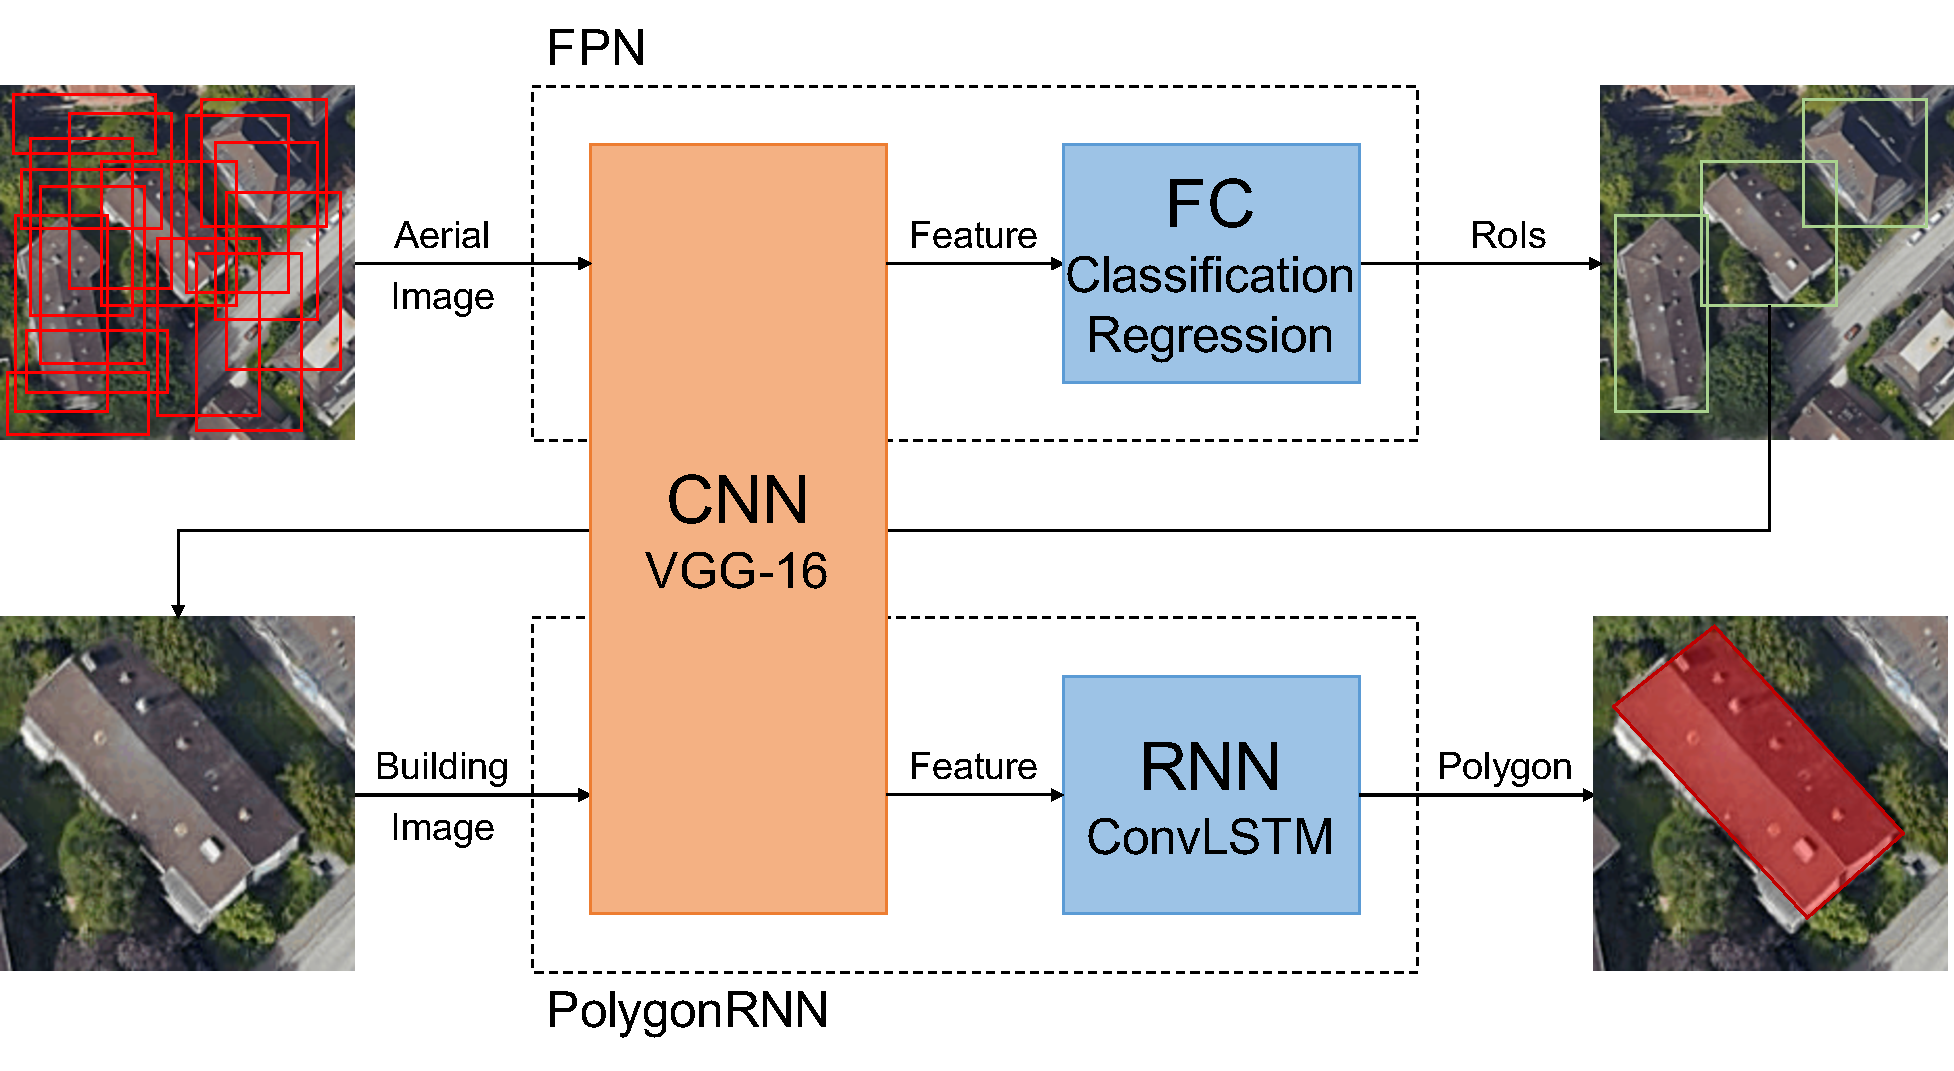
\includegraphics[width=\fig\textwidth]{3-16.pdf}
    \caption[\modelnameshort\ , hybrid version]{\modelnameshort\ , hybrid version.}
    \label{fig:hybmod}
\end{figure}

As a result, the training phase of the whole model \modelnameshort cannot be separated, and multi-task training is needed in this version. In general, multi-task training introduces network parameter sharing, which can reduce the model parameters, make the training phase better, and therefore improve the the model's prediction effect and accuracy. In addition, the model's generalization ability can be also improved through multi-task training.

\subsection{Hybrid Version with RoIAlign}\label{algmod}
Note that both two-step version and hybrid version do convolution for the aerial image and the building image respectively. However, we know that the building image is taken from the aerial image, so there is redundancy in the twice convolutions. Considering that we already have the feature map of the aerial image, it is unnecessary to do a second convolution since we can take the building feature from the corresponding position in the feature map of the aerial image, when given the RoI.

In Mask R-CNN, RoIAlign \cite{maskrcnn} is proposed to solve this kind of problem. Actually its previous version, RoIPooling \cite{fasterrcnn} is already used in Faster R-CNN. The role of RoIPooling is to pool the corresponding area in the feature map into a fixed-size tensor, so as to perform subsequent classification phase. The positions of the RoIs are usually obtained by regression of the model, which are generally floating numbers. In order to get fixed-size feature, RoIPooling has twice process of rounding these floating numbers: (1) Box boundaries are rounded to integers; (2) The region of box is divided into several cells, boundaries of each cell are rounded to integers. Actually we can also simply regard RoIPooling as a kind of nearest-neighbor interpolation. After twice rounding process, each cell has a certain deviation from its initial position, which will have negative effect on the accuracy of subsequent classification or semantic segmentation (only for Mask R-CNN). This problem is summarized as ``misalignment" in Mask R-CNN paper.

\begin{figure}[!h]
	\centering
	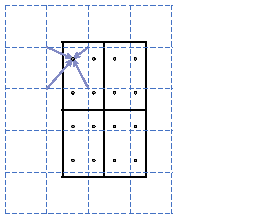
\includegraphics[width=\figfigfi\textwidth,angle=90]{3-18.pdf}
    \caption[Example of bilinear interpolation in RoIAlign]{Example of bilinear interpolation in RoIAlign. Image copyright owned by \cite{maskrcnn}.}
    \label{fig:roialg}
\end{figure}

In order to tackle the shortcomings of RoIPooling, Mask R-CNN introduces RoIAlign, using bilinear interpolation instead of rounding numbers. It can be used to obtain the value at the pixel whose coordinates are floating numbers, thereby transforming the pooling process into a continuous operation. Figure \ref{fig:roialg} shows an example of RoIAlign.


Therefore, we can simply apply the bounding boxes obtained from FPN calculation directly on the feature map by RoIAlign and send the pooled features to the RNN part of PolygonRNN. Figure \ref{fig:algmod} shows the model architecture of hybrid version with RoIAlign of \modelnameshort.

\begin{figure}[!h]
	\centering
	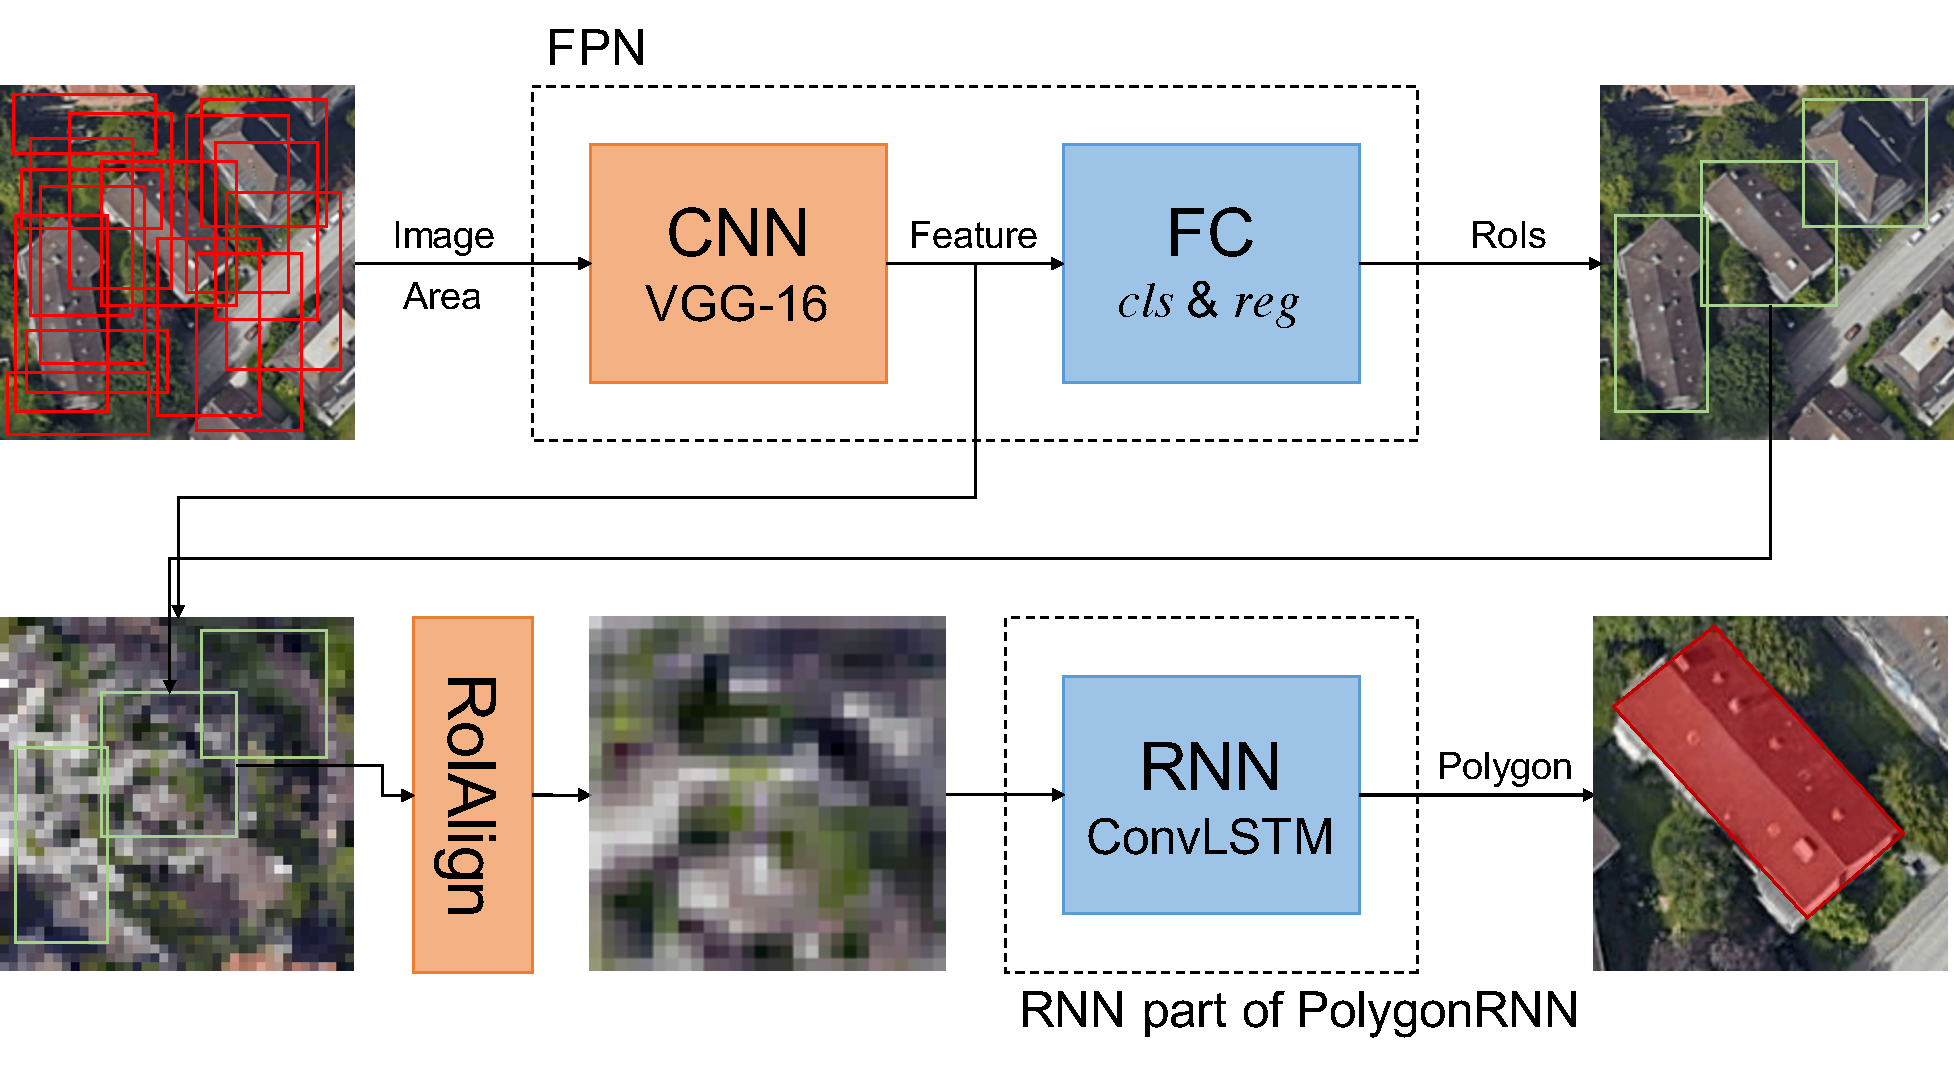
\includegraphics[width=\fig\textwidth]{3-17.pdf}
    \caption[\modelnameshort, hybrid version with RoIAlign]{\modelnameshort, hybrid version with RoIAlign.}
    \label{fig:algmod}
\end{figure}

As a result, VGG-16 is used only once and therefore it can speed up both training and prediction in theory. However, in practice, we usually resize the aerial image into a low resolution before feeding it to FPN, in order to make the network faster. Thus, the feature pyramid we obtain is at a ever lower resolution. If we directly use RoIAlign to get the building features, a lot of semantic information of the building would be lost. Hence, RoIAlign requires the input of aerial image with original resolution, and in this case, FPN would slow down. So here we think that this version will not have much improvement in speed. Therefore, due to the reason mentioned above and the time limitation of this thesis project, this version of \modelnameshort\ is not implemented yet, which would remain as future work. 

\subsection{Beam Search}\label{bmsrch}
In the prediction phase of \modelnameshort, the beam search algorithm is introduced, which is not used in original paper \cite{polygonrnn}. Beam search is a heuristic graph search algorithm, which is usually used when the solution space of a graph is relatively large. In order to reduce the space and time occupied by the search, at each step of depth expansion, some poor quality knots are cut off, and higher quality nodes are kept. This process can significantly reduce space consumption and improve time efficiency, but the disadvantage is that, there may be potentially optimal solutions discarded. Therefore, the search result is not necessarily the optimal solution. Experiments show that the introduction of beam search can tackle the problem of skipped vertex.

Figure \ref{fig:bmsrch} shows a single step of the beam search algorithm with beam width equaling to 3.

\begin{figure}[!h]
	\centering
	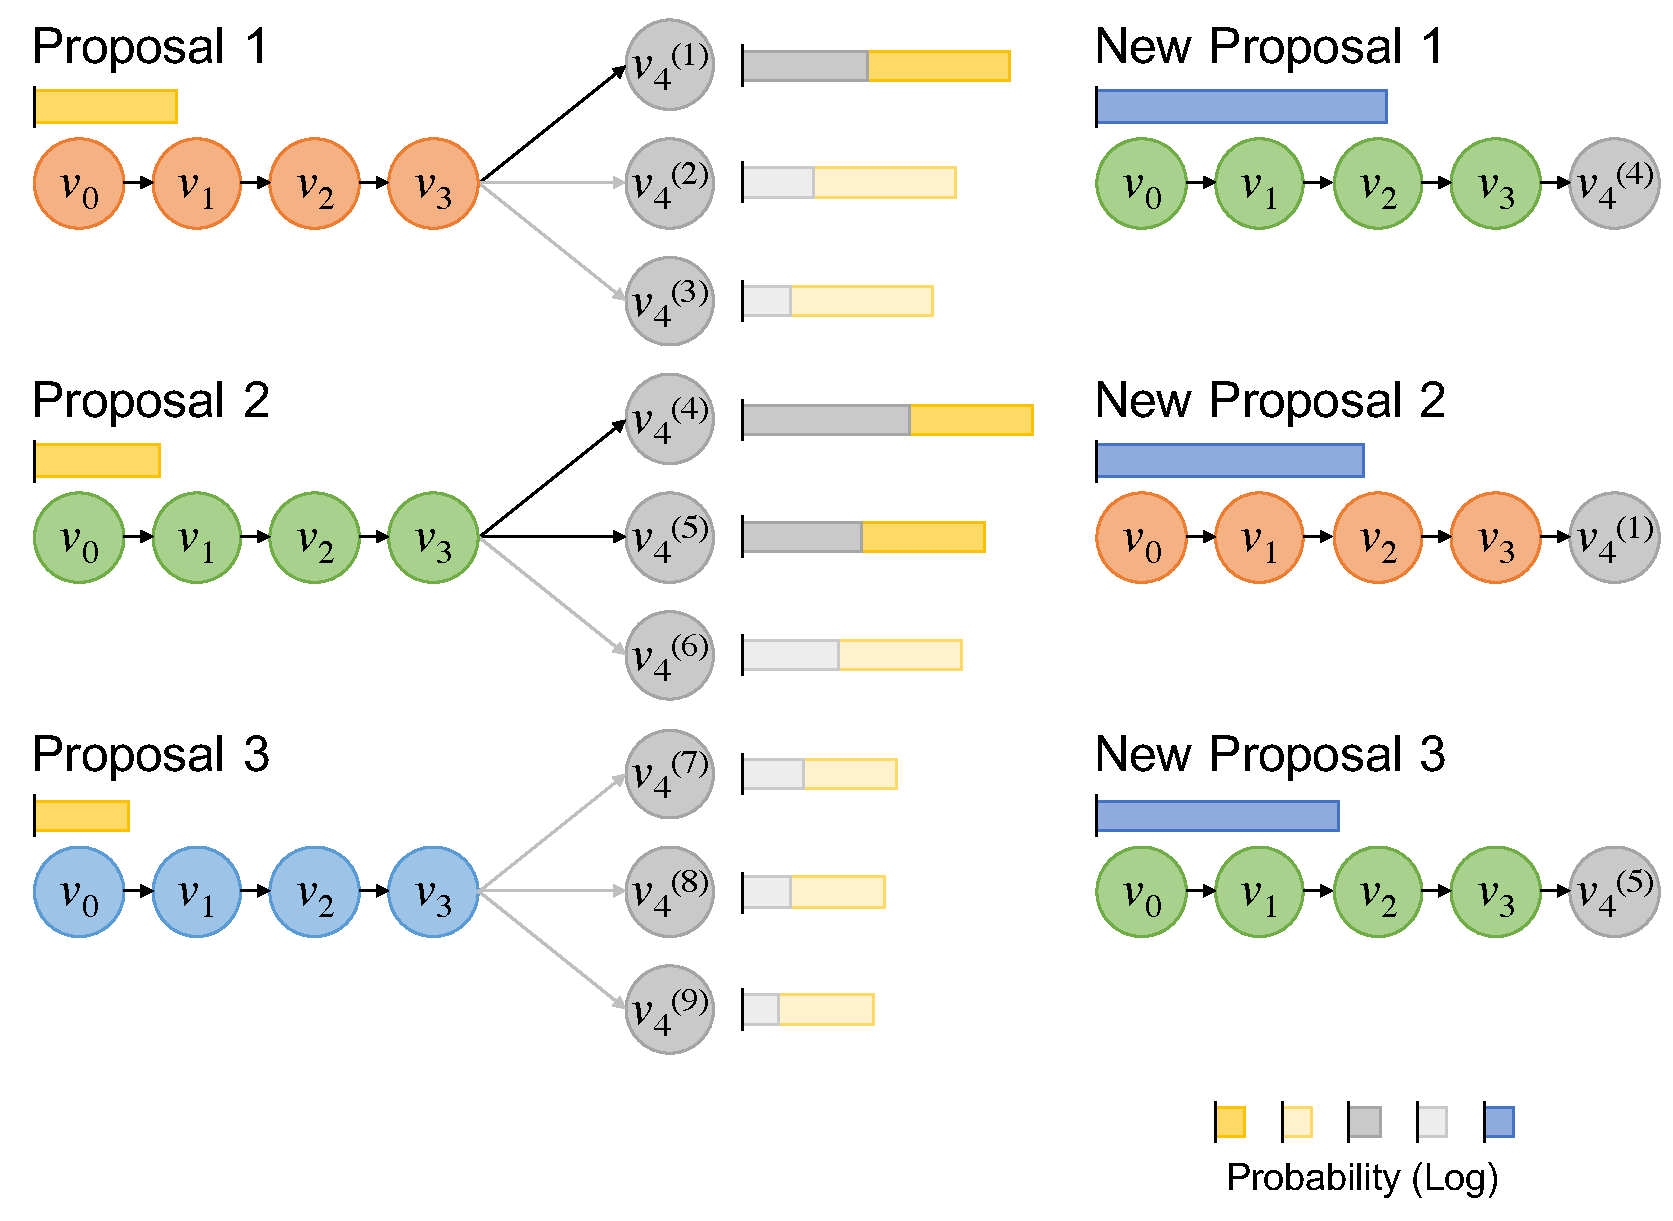
\includegraphics[width=\fig\textwidth]{3-19.pdf}
    \caption[Example of single step of beam search algorithm]{Example of single step of beam search algorithm. Suppose currently we have three proposals for the first four vertices, with its corresponding probability (in yellow). For each proposal, we compute the probability distribution (in gray or light gray) for the fifth vertex, and present top three with highest probability. Totally we have nine possible choices. For each choice, we compute its probability, which is the current one (in gray) plus (here using log probability, thus plus) the previous one. We take top three of these nine choices as our new proposals with new probability (in blue), and continue to the next loop.}
	\label{fig:bmsrch}
\end{figure}





